\documentclass[english]{lni}

\IfFileExists{latin1.sty}{\usepackage{latin1}}{\usepackage{isolatin1}}

\usepackage{graphicx}
\usepackage{wrapfig}
\usepackage{fancyhdr}
\usepackage{listings} %if lstlistings is used
\usepackage{changepage} %for changing topmargin on first page
\usepackage{amsmath, amssymb, gensymb}
\usepackage[figurename=Abb., tablename=Tab., small]{caption}[2016/04/20]
\renewcommand{\lstlistingname}{List.}    % Listingname hei�t nun List. 
\renewcommand{\paragraph}[1]{{\bf#1}}

%Beginn der Seitenz�hlung f�r diesen Beitrag
\setcounter{page}{1}

%Kopfzeileneinstellungen
\pagestyle{fancy}
\fancyhead{}
\fancyhead[L]{\small Paper handin for:\hspace{5mm} BIOSIG 2016\\Author:
%							\hspace{17mm}Magnus {\O}verb{\o}}
							\hspace{17mm}[FIRST NAME] [LAST NAME]}
\fancyhead[R]{\small Page \thepage}
\fancyfoot{}
\renewcommand{\headrulewidth}{0.4pt}
\setcounter{footnote}{0}

%\author{Magnus {\O}verb{\o}\footnote{NTNU, Gj{\o}vik, Norway, magnus.overbo@stud.ntnu.no}}
\author{[First Name] [Last Name]\footnote{[SCHOOL], [LOCATION], [COUNTRY], [EMAIL]}}
\title{Distribution Assessment of Iris Quality Metrics\\for Visible Wavelength
photos}


\begin{document}
\maketitle
\setcounter{footnote}{2}

\begin{abstract}
This paper explores how different image metrics differs in the ability 
to classify periocular images in the visible wavelength spectrum.  There 
were two extraction tools created for this paper. BIQA\cite{biqa} and
IQA\cite{iqa}.  The metrics extracted was then tested for their ability classify
the data sets into "good" and "bad" images.  BIQA is based on the works of
various authors and IQA is a reverse engineering of Hugo Proencas 
paper\cite{hugo}.

The results shows that several metrics were not applicable for classification of
images focusing on the periocular region and some performed very well for
classifying the data set and is summarised in table \ref{tab:appl} in the
conclusion.

\end{abstract}

\begin{keywords}
	iris, visible wavelength, quality metrics, quality assessment, classification,
	svm
\end{keywords}


\section{Introduction}
Current quality metrics(QM) used in iris recognition is based on the Near
Infra-Red (NIR) spectrum.  This paper explored several methods to extract QMs
from an image in the visible wavelength(VW) spectrum. The extracted metrics is 
then used as input to an SVM classifier before the metrics ability to classify
the data set is analysed.

This project was done due to the increasing popularity of using iris recognition
on photos in the VW spectrum.  Therefore it is important to verify the quality
of the image, which this paper has explored.  However, the classification has
not been run through a comparison test because it is out of the scope.

The paper created two tools for extracting QMs from periocular images. "Blind 
Image Quality Assessment" (BIQA) \cite{biqa} extracts twenty-three metrics, of
which a subset are used for assessment.  "Iris Quality Assessment" (IQA)
\cite{iqa} is a reproduction of Hugo Proenca paper "Quality Assessment 
of Degraded iris images acquired in the visible wavelength" \cite{hugo}. IQA 
collects the same metrics as Proenca, except for the iris pigmentation metric.


\section{Related work}
This paper has explored and developed two systems for extracting blind quality 
features from periocular images captured in the visible wavelength (VW)
spectrum.
The resulting features is then run through a SVM for training and classification
where the training set was manually classified.

First off, BIQA\cite{biqa} is the system which was based upon metrics gathered
from the ISO standard\cite{iso} and various methods as detailed below. Which
include the tools NIQE \cite{niqe}, BRISQUE \cite{brisque}, NSS \cite{nss},
JP2KNR \cite{jp2knr} and BIQI\cite{biqi}.

It has already been done work on blind image quality assessment, especially the 
University of Texas\footnote{University of Texas:
\texttt{http://live.ece.utexas.edu/research/Quality/index.htm}}.
The paper has implemented the following blind image quality assessment (BIQA)
tools that has been published and are publicly available; BRISQUE, JP2KNR
Quality metric, BIQI, and NIQE.

Anish Mittal, Rajiv Soundararajan, and Alan C. Bovik\cite{niqe} has developed a
blind image quality model called "Natural Image Quality Evaluator" (NIQE) which
runs through an image and assess its quality based on a statistical models for
the natural scene statistics (NSS) based on L. Ruderman article "The Statistics
of Natural Images"\cite{nss}.

Anish Mittal, Anush K. Moorthy, and Alan C. Bovik has proposed a BIQA model
operating on the spacial domain, "Blind/Referenceless Image Spatial Query
Evaluator" (BRISQUE)\cite{brisque}.  This model focuses on using scene
statistics to quantify possible losses of "naturalness", resulting in a holistic
measure of quality.

Hamid R. Sheikh, Alan C. Bovik and Lawrence Cormack \cite{jp2knr} has proposed a
method of applying NSS to measure the quality of images compressed using wavelet
based image compression.  The hypothesis they started with was that the
compression results in loss of quality that can be related to human perception
of quality.

The tool "Blind Image Quality Index" (BIQI)\cite{biqi} developed by Anush
K. Moorthy and Alan C. Bovik is focusing on assessing the distortions
in an image. BIQI is based on a trained classifier that does not require any
prior knowledge once its trained and can be extended to assess any type of
distortion.  As with the NIQE\cite{niqe}, BIQI is based on an NSS model.

For the other metrics being implemented in this project, I have relied on the
ISO 29794-6 standard\cite{iso}.

For the second tool, the Iris Quality Assessment (IQA)\cite{iqa}, I've reversed
engineered Hugo Proencas paper\cite{hugo}.  Many of the points in this
paper are overlapping with the metrics from the ISO standard.  Hugo proposes to
use seven metrics as the basis for classification. This paper implemented
six of them.



%\input{chapters/}

\section{Software}
\label{sec:software}
This section explains how the tools created in this paper works and calculates
its metrics.
BIQA and IQA were developed as part of two separate projects and joined
together for this paper.  BIQA\cite{biqa} was developed to explore how well 
the metrics in the ISO 29794-6 \cite{iso} is for classification
purposes. The metrics are summarised in table \ref{tab:indclas}.
The IQA\cite{iqa} project was to reverse engineer the methods proposed by Hugo
Proenca\cite{hugo} which utilised a set of metrics to estimate the quality of 
the iris images in visible spectrum. This tool was hard to reverse because it is
proprietary software.


\subsection{Iris Quality Assessment (IQA)}\label{sec:iqa}
\paragraph{Area Assessment}
The area assessment is based on the assessing how many pixels covering the iris
are considered to be noise free and are calculated:
\begin{align}
A = \Sigma_Y\Sigma_X( \forall_{x,y} I_{mask}\notin\{0\} ) 
\end{align}


\paragraph{Off-Angle}
Data from the OSIRISv4.1 generated parameter file, containing all coordinates of
the iris and pupil are, is parsed. This generates two convex hulls(CH) for the 
iris and pupil area. This method applies to both the iris and the pupil CH. Go 
through each set of coordinates in the CH and calculate the angle, rotate the
CH accordingly and calculate the area of the CH using a bounding box. Using 
the width and height of the rotated CH. When all angles has been tested, one has
found the angle where the CH covers the smallest area.
Then one calculates the angle of the bounding box, before calculating the alpha 
angle and Theta-angle(in degrees) using. 
\begin{align}
	A_a &= (1 - \frac{Len_{min}}{Len_{max}})\\
	\Theta &= tand( atan2d( \frac{\sin(A_{min} \cdot B_w)}{Len_{max}}, \frac{\cos(A_{min} \cdot B_W)}{Len_{min}} )
\end{align}


\paragraph{Focus}
The focus assessment first removes all unwanted pixels by "removing" the area
which is not the iris by using the mask generated by OSIRIS. The focus 
assessment then uses the high-pass filter to create a sharper image
\footnote{Code originates from University of Regina: \texttt{http://www.cs.uregina.ca/Links/class-info/425/Lab5/}} 
which is used to calculate the focus assessment.
\begin{align}
M = \Sigma_Y\Sigma_X( abs( F_{shift}( F_{trans}( I_{sharp} ) ) )^2 ) 
\end{align}


\paragraph{Motion Blur}
Motion blur is calculated on the noise-free area of the iris by "removing" the 
remainder of the image by applying the iris mask.  The focus assessment is
performed by rotating the image and iris-mask at fixed increments before running
it through a Fourier transform (Eq. 5). The output is run through the a focus
assessment returns the magnitude. After all rotations has been tested $A\in
[0,2,..,180]$, it calculates the magnitude of the motion blur with
$M_{max}-M_{min}$, and the angle of motion is where the min magnitude occurred.
\begin{align}
abs( F_{shift}( F_{trans}( I ) ) )^2 
\end{align}



\paragraph{Pupil Dilation}
The dilation of the pupil is assessed by the ration of what is considered the
area of the pupil, to what is considered the iris area.
\begin{align}
A_p = \frac{Pupil_{area}}{Iris_{area}} 
\end{align}




\subsection{Blind Image Quality Assessment (BIQA)}\label{sec:biqa}
\vspace{-3mm}
BIQA is based on metrics described in the ISO standard 29794-6\cite{iso},
and four 3rd party tools; the NIQE\cite{niqe}, BRISQUE\cite{brisque},
JP2KNR\cite{jp2knr}, and BIQI\cite{biqi}.
Table \ref{tab:indclas} shows the different metrics retrieved from
the images, marked with "BIQA". Not all of metrics gathered are used for the process of training and
classifying a SVM, but may be used later and is currently used for retrieving 
and calculating the other ISO metrics.



\paragraph{Usable Iris Area}
The usable iris area, as standardised in section 6.2.1 of the ISO 29794-6
\cite{iso}, is the non-occluded area of the iris.
The method used in this paper is a simple calculation of calculating the
percentage iris that is missing due to the size of the pupil.
\vspace{-3mm}
\begin{align}
	UIA &= (1-\frac{N_{occluded}}{N_{iris}} ) \cdot 100
\end{align}



\paragraph{Iris-Pupil Contrast}
The contrast between the iris and pupil is stated in section 6.2.3 of ISO
29794-6\cite{iso}. 
The implementation uses data sampling from the iris and pupil 
area, not the entire area.  The iris and pupil values are selected by
calculating the median values, then calculating the contrast using these values.
In addition the Weber ratio formula, it implements the same formula as for the 
iris-sclera contrast. Giving an extra metric.
\vspace{-3mm}
\begin{align}
	weber\_ratio &= \frac{|iris - pupil|}{1 + pupil}	\\
	IPC &= \frac{weber}{0.75 + weber}
\end{align}



\paragraph{Iris-Sclera Contrast}
The ISO standard provides a method to compute the contrast between the iris area
and the sclera. By measuring the lightness of the sclera area and the iris 
separately one can compute the contrast ratio, using the formula from the ISO
standard 29794-6 section 6.2.2 \cite{iso}.  This papers approach is the same as
for iris-pupil contrast by using samples instead of the entire area. BIQA then
uses the median values of the samples.
\vspace{-3mm}
\begin{align}
	ISC = \frac{|sclera - iris|}{sclera + iris} \cdot 100
\end{align}




\paragraph{Grey Scale Utilisation (GSU)}
The GSU is measured as the entropy of grey scale pixels and represents
the number of bits needed to represent the image.  The entropy is calculated as
below. Where, $p_i$ is the number of pixels with a given value, $p$ is the
number of all pixels and $P(p_i)$ is the probability of $p_i$ occurring in the 
pixel set.  BIQA calculates the GSU for both the entire image and a subset of 
the iris, giving two separate metrics.
\vspace{-3mm}
\begin{align}
	H &= -\Sigma p_i \log_2 p_i \\
	P(p_i) &= \frac{ \Sigma{p_i} }{ \Sigma{p} }
\end{align}



\paragraph{General Metrics}
In addition to the more specific ISO standard requirements for image quality,
the ISO standard\cite{iso} sets forth additional metrics to assess the quality
of the iris image captured.  Which some are extracted, but not used for this
paper.



%\section{Support tools}
\label{sec:support}

While developing the main tools, I was forced to develop some support tools in
order to manage the databases of images, generating Matlab files, classification
and automation of the segmentation processing with OSIRIS\cite{osiris}.


\subsection{WebIIC}
\label{sec:webiic}
Web Iris Image Classifier (WebIIC)\cite{webiic} performs the task of performing
manual classification of images in the database.  The WebIIC has three tasks;
load the list of images into the database, classification of images, and manual
positioning of the right pupil, left pupil and left iris. These points must be
aligned align along the centre of the pupil along the Y-axis.

The latter task is because of future ability to redo segmentation with fixed
values for pupil and iris size and position.  OSIRIS v4.1 does not allow for
this at the current time.

WebIIC eases the process of classifying images manually significantly and makes
the classification random.  This because it selects the subset of all images not
yet classified, then performs a random selection of one image from this subset.
Which is then loaded into the web frontend for classification or manual point
selection.

The classification allows an image to be set to either of three values,
"Not Classified", "Good", "Bad" or "Error". The error class is used for very
poorly classified images, but is not used in this project.

\begin{description}
\item [Good] The image receives a classification of "1" in the "CLASS" field.
\item [Bad]  The image receives a classification of "0" in the "CLASS" field.
\item [Error] The image receives a classification of "-2" in the "CLASS" field.
\item [Skip] Nothing is done and the image is skipped, maintain current "CLASS"
	which is by default "-1".
\end{description}



\subsection{DBIris}
\label{sec:dbiris}

DBIris\cite{dbiris} consists of several scripts, with the goal of generating a
file containing all the databases.  Which contains all the images successfully
processed by OSIRIS v4.1\cite{osiris}.  The finished files are to be used by
webIIC for loading images into its database and by BIQA and IQA to load images
for metric extraction.

The first script to use is the "osiris\_gen.py" which takes a single file
containing the full path of each image to process.  This will run each image
through the defined configurations for OSIRIS, until the iris is found and
segmented or no more configuration files are available. The resulting images are stored in
the defined folder according to the OSIRIS configuration files.

The second script to run is the "dbGenerator.py" which takes the same file as
"osiris\_gen.py" uses, an integer stating how many databases to create, the path
to the Matlab file containing the databases and the path to the file to be used
by webIIC.

The third script, which is reserved for the future, is the "osiris\_man\_gen.py"
which generates the segmented iris and pupil image(without occlusion assessment)
and the mask for iris area.

DBIris also stores all the images in two folders, the "db\_periocular" and
"img\_processed" by default.  Making it easier to mange for all applications by
having a centralised repository.








\section{Testing Methodology}\label{sec:test}
To perform classification 625 "good" and 560 "bad" images was manually
classified using webIIC \cite{webiic} and used for training the support vector
machine (SVM). The testing was done by using an SVM to classify the individual
metrics on the data sets to ascertain the distribution then analyse the results.

After randomly exploring these data sets, I've noticed a large portion of the
images are of lower quality. After classification the result was plotted using a
scatter-plot diagram for illustrative purposes which shows the overlap and can
be used for further analysis.




\section{Data sets}\label{sec:dataset}
Three databases was used for this paper and consisted of totally 11.292 images
of the periocular region of the face.  Originally it was 12.689, but some images
could not be used because of errors occurring in OSIRIS v4.1\cite{osiris}.
The data sets which has been used in this paper is the UBIRIS.v2\cite{ubiris},
MICHE\cite{miche} and an independent data set captured at Norwegian University of
Technology and Science (NTNU).

UBIRISv2. consists of images captured at a distance during movement. It was 
created by Hugo Proenca, et al \cite{ubiris}. The images are 600x400 pixels and
of varying quality. Most images are focused on the periocular region, but
several have failed to capture the iris.  The data set I've used contained a
total of 11101 images.

The MICHE\cite{miche} data set contains large images of the periocular region. 
The images are captured in various environments using either an iPhone 5 or 
Samsung Galaxy using both cameras on each phone and in two environments for each
camera. MICHE contains images of varying quality and resolution. In total I've
used 1536 of the images from MICHE.

The last data set is generated at NTNU and contains 52 high quality images of
uniform lighting.


\section{Data Analysis}\label{sec:analysis}
\vspace{-3mm}
This section explores how the different metrics retrieved are distributed for
the images.  For all figures, the data is plotted along the X-axis with the
number they are in the resulting matrix and their value along the Y-axis.
During metric extraction the BIQA scaled images down to a width of 600px, while
IQA did not scale these images.  This led to some issues, for focus assessment
some images has a larger focus value.

In the following analysis it tries to find metrics with good statistical
properties for classification. This requires it to have clear groupings which
yields good inter and intra class grouping. Meaning "good" images should be
grouped together and clearly differ from "poor" images.

\subsection{IQA Metric analysis}
\vspace{-3mm}
\subsubsection{IQA - Iris Area metric}\vspace{-5mm}
	\begin{wrapfigure}{R}{0.325\linewidth}
		\centering
		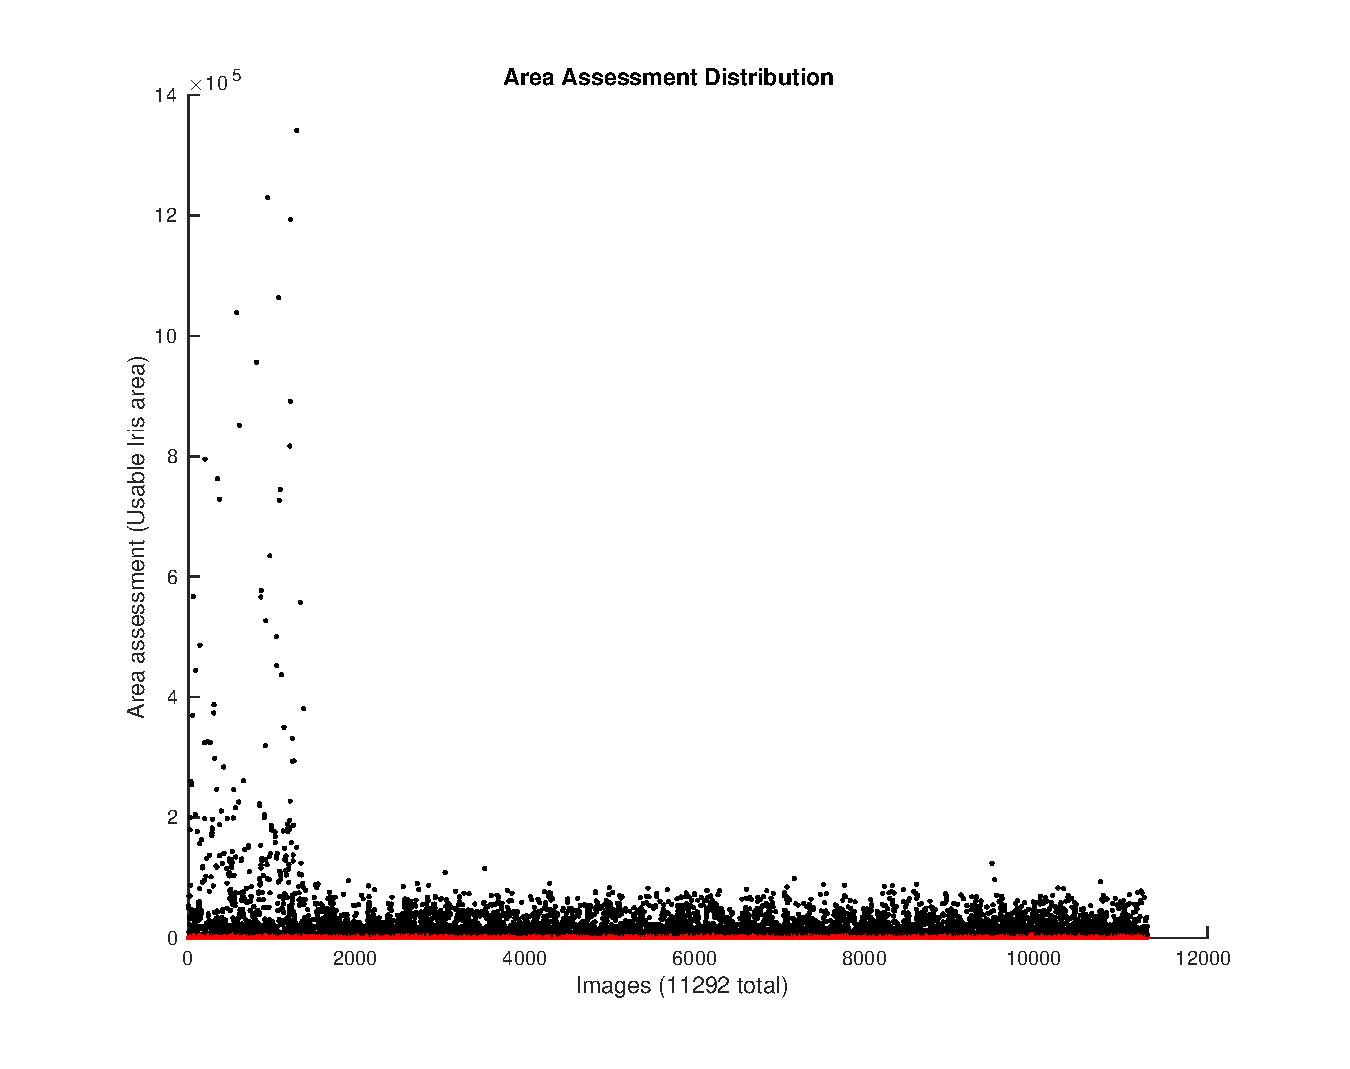
\includegraphics[height=2cm, width=5cm]{pics/dist_area_assess}
		\caption{Usable area\cite{hugo}}
		\label{fig:area}
	\end{wrapfigure}
The usable area metric is not affected by the resolution of the image and its
value is the number of pixels in the noise-free iris area.
In figure \ref{fig:area}, a clustering close to the bottom implies a
distribution weighted to the lower end of the spectrum. An higher values clearly
differing from the initial clustering.  This should mean that it is possible to
differentiate between inter-class values during classification for the metric.

\subsubsection{IQA - Iris Off-Angle Metric}\vspace{-5mm}
	\begin{wrapfigure}{R}{0.325\linewidth}
		\centering
		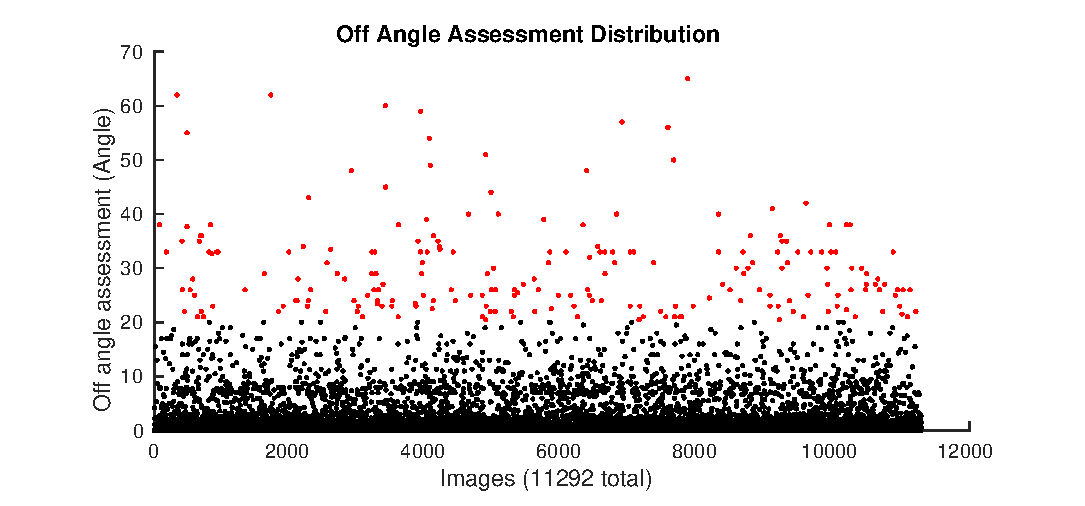
\includegraphics[height=2.25cm, width=5cm]{pics/dist_off_angle_deg_2}
		\caption{Off-angle assess. \cite{hugo}}
		\label{fig:ang}
	\end{wrapfigure}
The off-angle metric states how much the iris is rotated since a non-direct gaze
into the camera will make it oval and rotate it slightly. In figure
\ref{fig:ang} the angle lies between 0\degree and 85\degree.
5\degree-10\degree seems to be outside the normal distribution. In the figure 
angles above 20\degree has been marked as "bad" angles, because they are far
outside the normal distribution.  There is a large inter class distance which
suggests a good possibility to differentiate the metrics. 

\vspace{-5mm}
\subsubsection{IQA - Focus Metric}\vspace{-5mm}
	\begin{wrapfigure}{R}{0.325\linewidth}
		\centering
		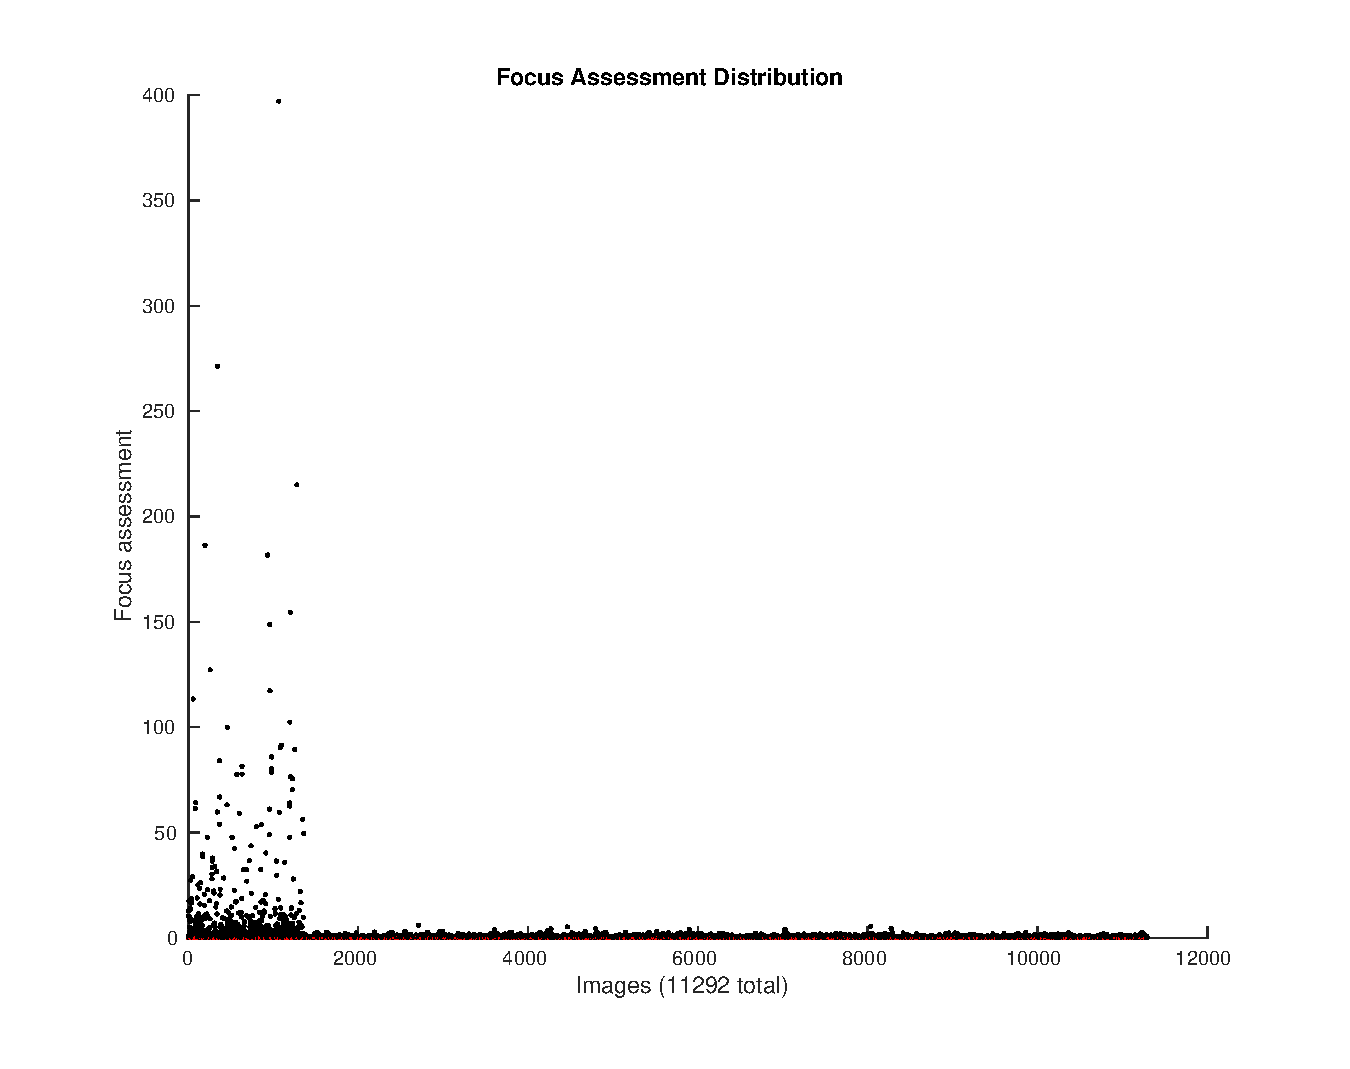
\includegraphics[height=2cm, width=5cm]{pics/dist_focus_assess}
		\caption{Focus assessment \cite{hugo}}
		\label{fig:focus} 
	\end{wrapfigure}
The focus metric is dictated by the relative magnitude to the mean value.
Because the images were not scaled to equal size some images has higher values
than the rest.  It also shows that there are images with low focus in the subset
as well.  The mean value is represented as the value 1, all values above 1 is
therefore considered to be of better focus than those below.

\vspace{-5mm}
\subsubsection{IQA - Motion Blur Metric}\vspace{-5mm}
	\begin{wrapfigure}{R}{0.325\linewidth}
		\centering
		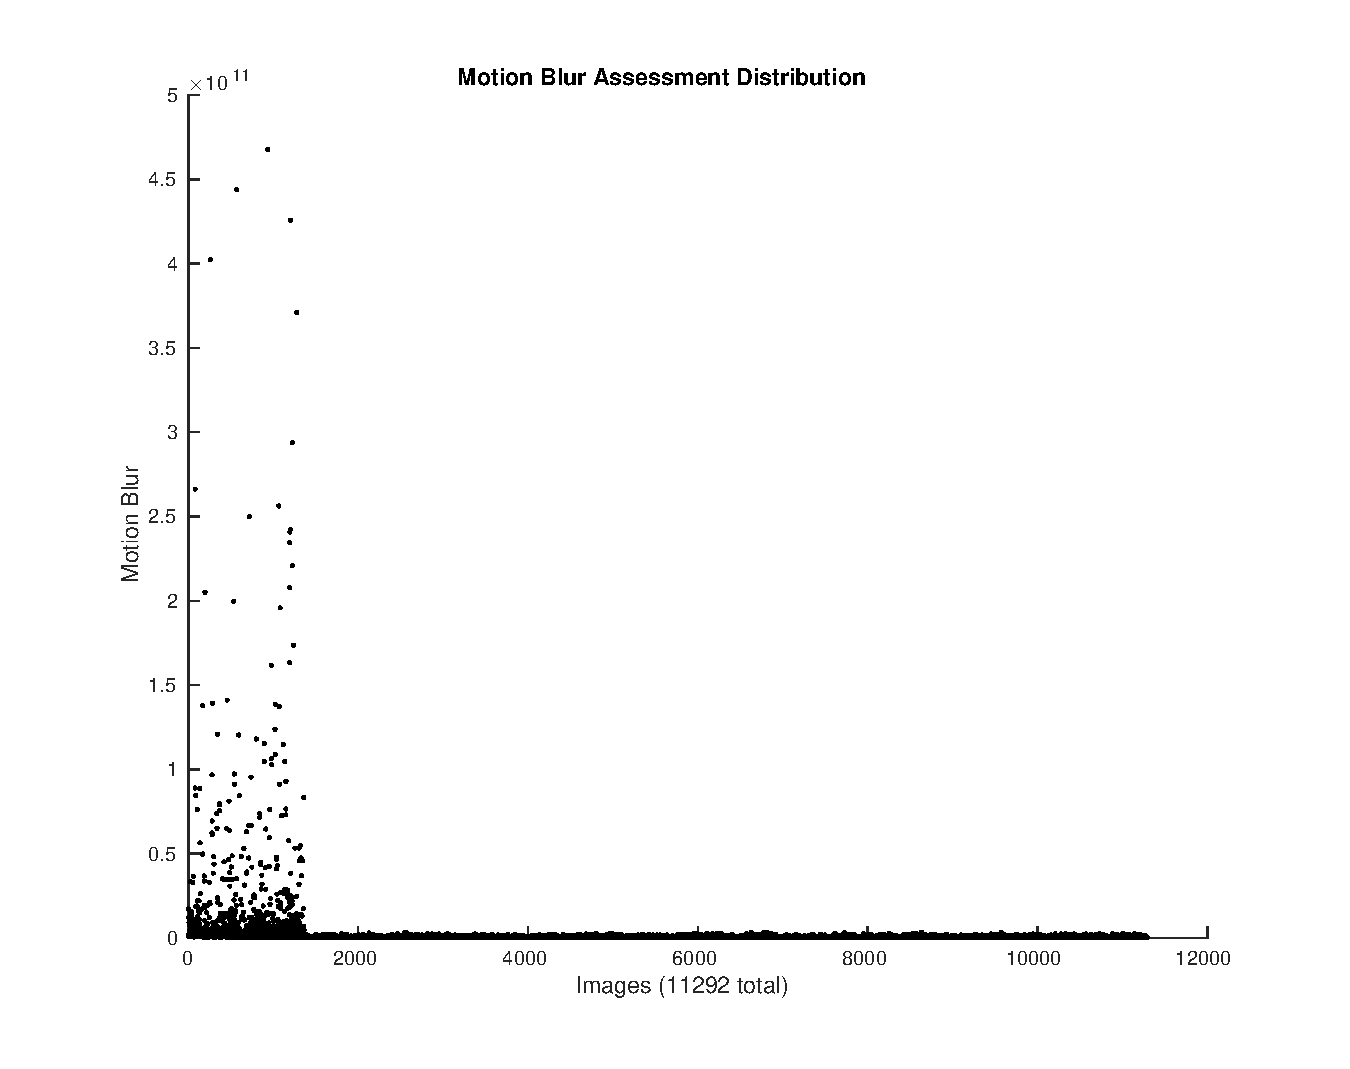
\includegraphics[height=2cm, width=5cm]{pics/dist_motion_blur_mag}
		\caption{Motion blur mag. \cite{hugo}}
		\label{fig:motion}
	\end{wrapfigure}
Motion blur is dictated by angle and magnitude of Fourier spectrum. This paper 
only evaluates the magnitude, where a higher value with more blur.
As for focus assessment, the same problem occurs for motion blur
assessment, figure \ref{fig:motion}.  The higher resolution images seems to have
much more blur than the than the UBIRIS data sets, suggesting  that the metric
may not be usable.

\vspace{-5mm}
\subsubsection{IQA - Pupil Dilation Metric}\vspace{-5mm}
	\begin{wrapfigure}{R}{0.325\linewidth}
		\centering
		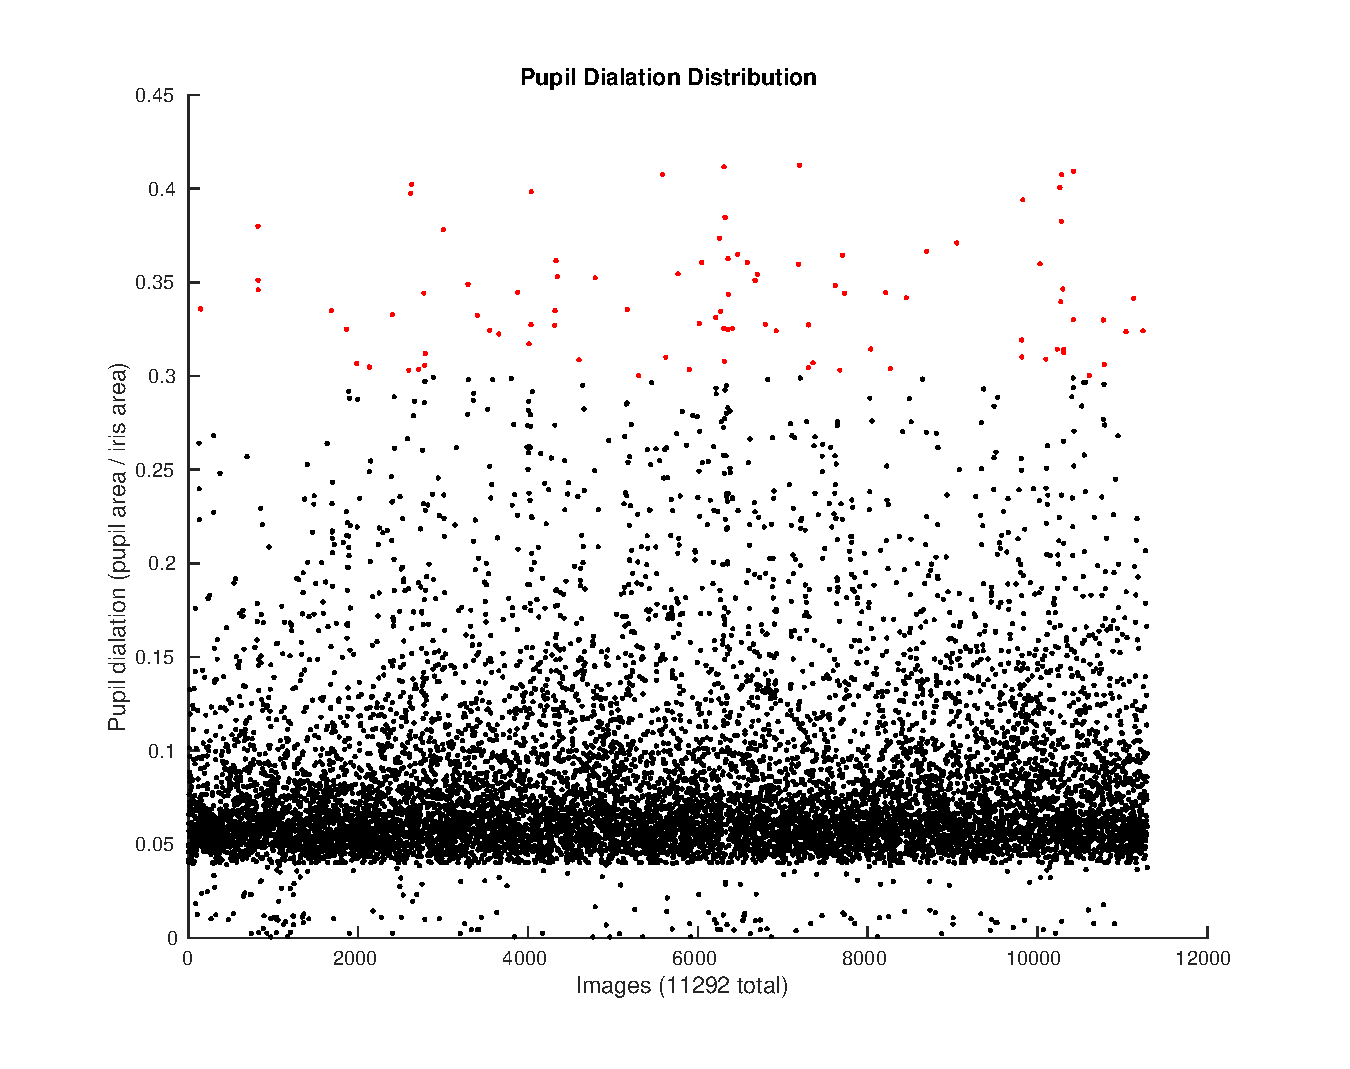
\includegraphics[height=1.5cm, width=5cm]{pics/dist_pupil_dilation_ratio}
		\caption{Pupil to iris ratio \cite{hugo}}
		\label{fig:ratio}
	\end{wrapfigure}
Figure \ref{fig:ratio} shows a very clear normal distribution which is equal
for all images.  This suggests that there is a good chance of performing
classification on this metric. This is however not likely because during
classification, the pupils where not distinctively larger for bad images.



\clearpage
\subsection{BIQA Metric analysis}
\vspace{-3mm}
\subsubsection{BIQA - Usable Iris Area Metric}\vspace{-5mm}
	\begin{wrapfigure}{R}{0.325\linewidth}
		\centering
		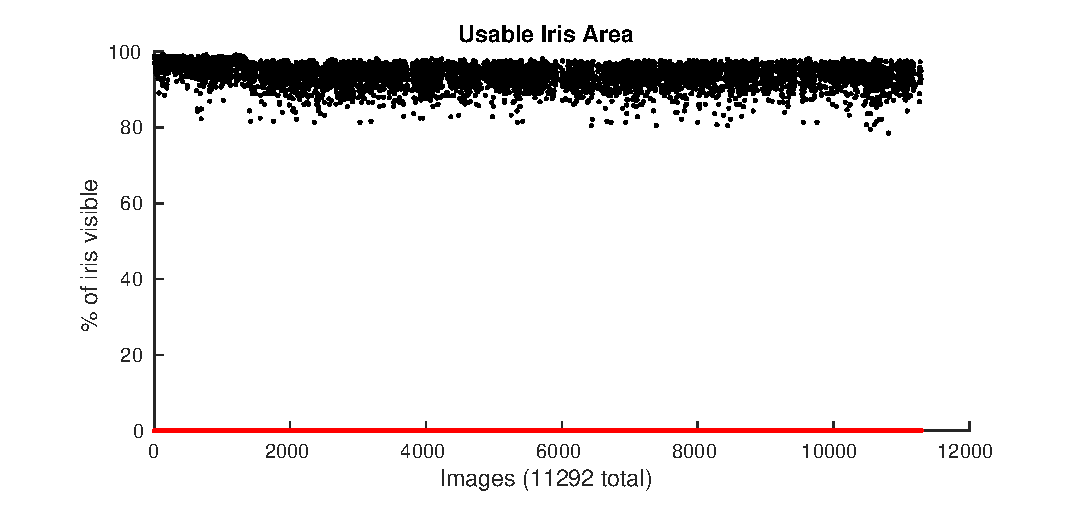
\includegraphics[height=2.25cm, width=5cm]{pics/biqa_dist_uia}
		\caption{Usable iris area \cite{iso}}
		\label{fig:uia}
	\end{wrapfigure}
The usable area metric differs from pupil dilation metric by incorporating
occlusions. This project did not implement this, meaning it is almost equal to
the pupil dilation metric.  This metric is the iris area minus the pupil area.
In figure \ref{fig:uia}, one can see that all the images is clustered to the top
which has a tight grouping making it hard to differentiate. Except for the
images which was unable to retrieve the metric from.


\vspace{-5mm}
\subsubsection{BIQA - Pupil-Iris Contrast Metric}\vspace{-5mm}
	\begin{wrapfigure}{R}{0.325\linewidth}
		\centering
		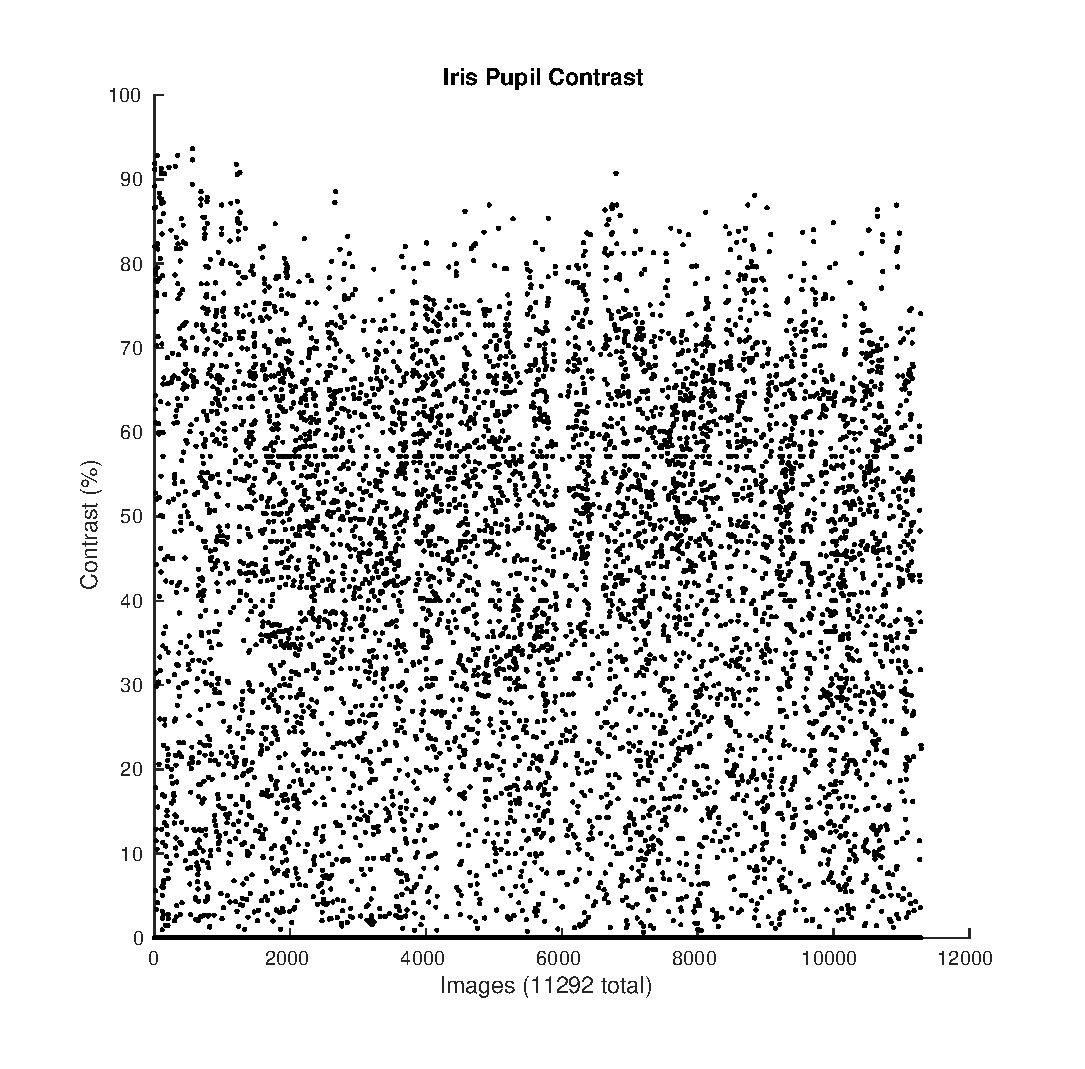
\includegraphics[height=1.25cm, width=5cm]{pics/biqa_dist_ipc}
		\caption{Pupil-iris contrast \cite{iso}}
		\label{fig:ipc}
	\end{wrapfigure}
The ISO standard sets forth the metric of pupil-to-iris contrast. In figure
\ref{fig:ipc}, one can see that this value is sparsely spread out. This could
state that there is a separation between different types of irises, or that
there is no definitive patterns to classify by.


\vspace{-5mm}
\subsubsection{BIQA - Iris-Sclera Contrast Metric}\vspace{-5mm}
	\begin{wrapfigure}{R}{0.325\linewidth}
		\centering
		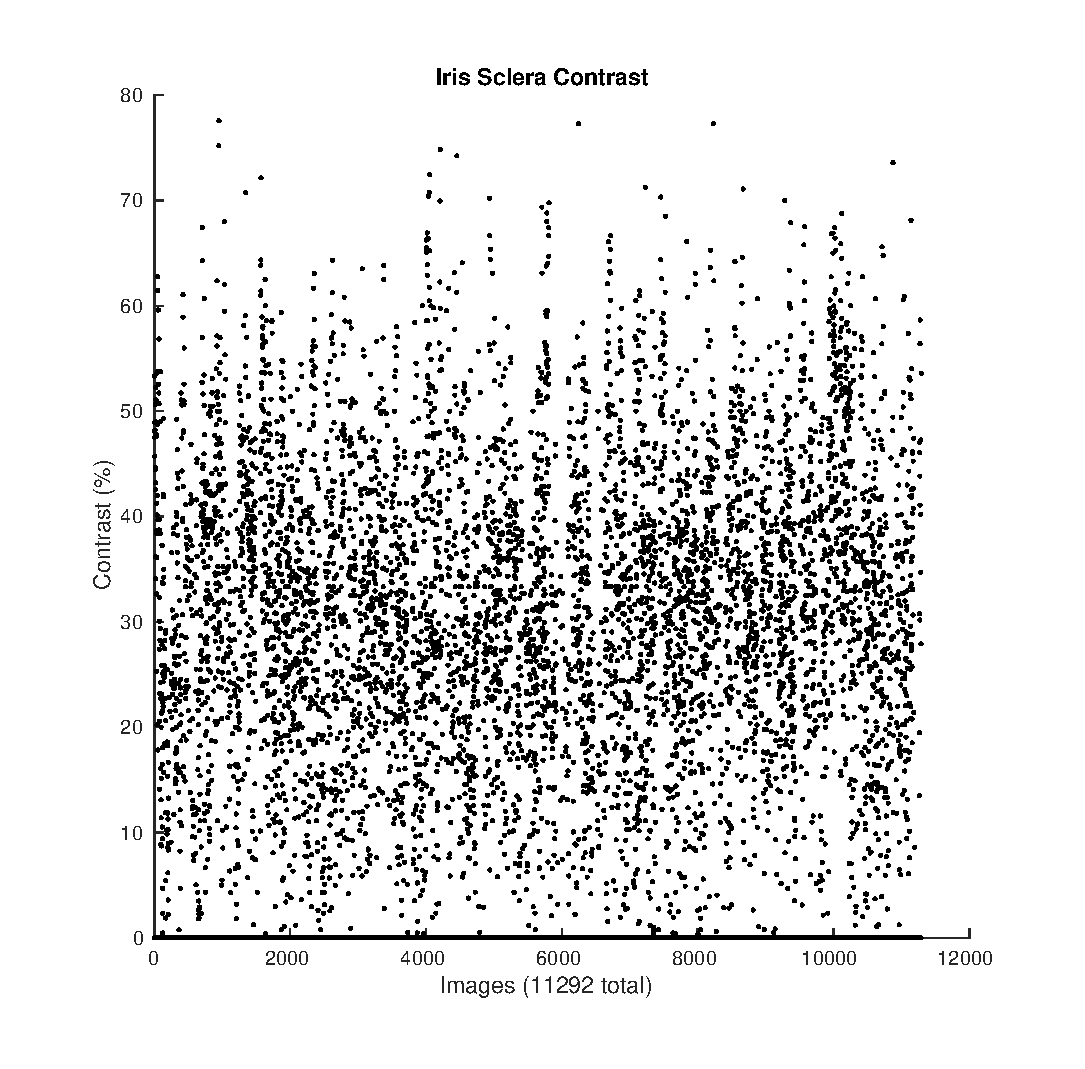
\includegraphics[height=1.25cm, width=5cm]{pics/biqa_dist_isc}
		\caption{Iris-sclera \cite{iso}}
		\label{fig:isc}
	\end{wrapfigure}
The ISO standard sets forth the metric of iris-to-sclera contrast. In figure
\ref{fig:isc}, one can see that this value is sparsely spread out. Just like the
iris-to-pupil contrast.  This could also  mean that is or is not at separation
that divides the different intra class types of contrasts.


\vspace{-5mm}
\subsubsection{BIQA - Pupil/Iris Ratio Metric}\vspace{-5mm}
	\begin{wrapfigure}{R}{0.325\linewidth}
		\centering
		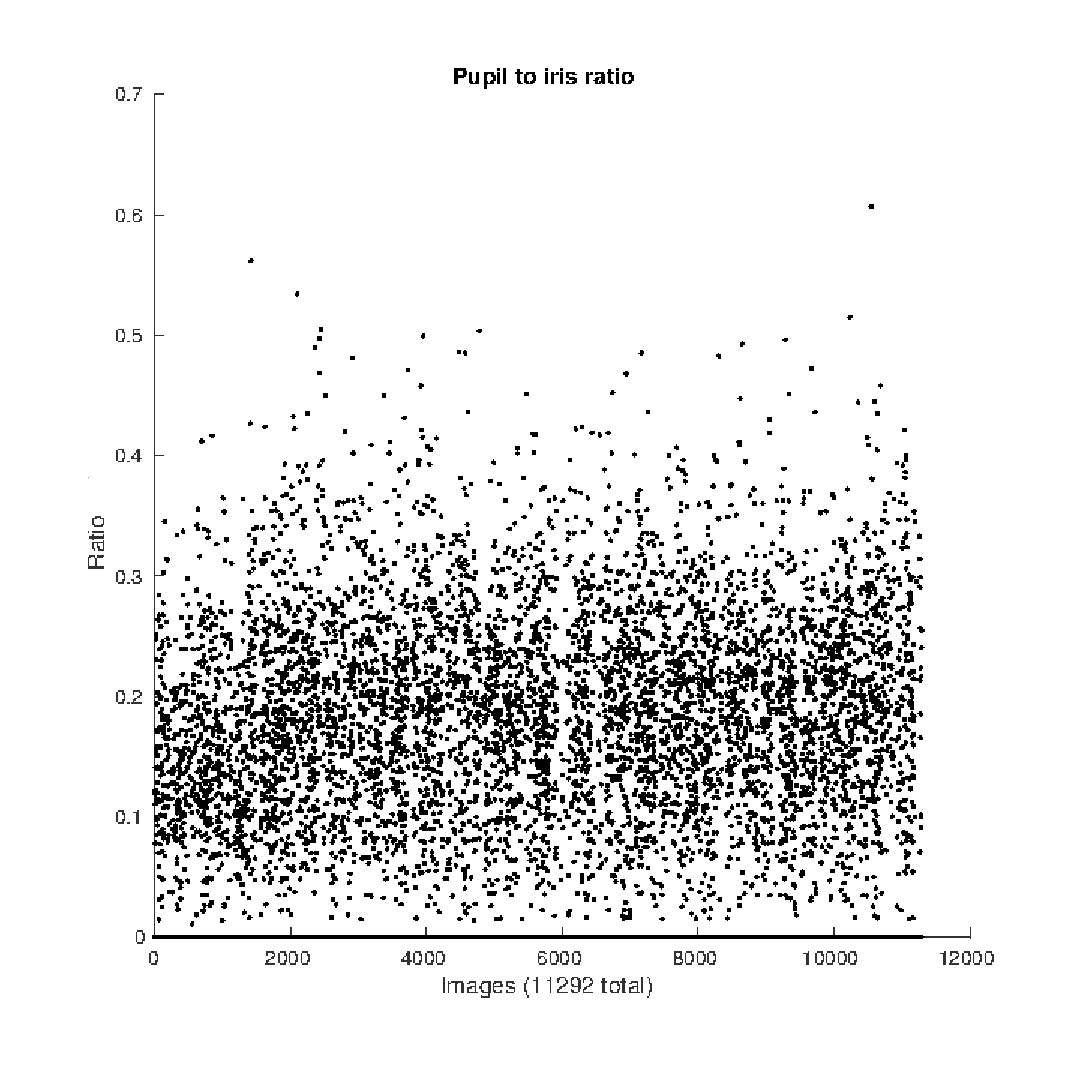
\includegraphics[height=1.25cm, width=5cm]{pics/biqa_dist_pup_ir_ratio}
		\caption{Pupil-iris ratio \cite{iso}}
		\label{fig:pir}
	\end{wrapfigure}
The ISO standard dictates this calculation.  As seen in figure \ref{fig:pir} 
there is a uniform distribution which appears to be loosely scattered throughout
the data sets.  It is however somewhat centralised around 0.1 and 0.2, but not
very distinctively.


\vspace{-5mm}
\subsubsection{BIQA - Grey Scale Utilisation Metric}\vspace{-5mm}
	\begin{wrapfigure}{R}{0.325\linewidth}
		\centering
		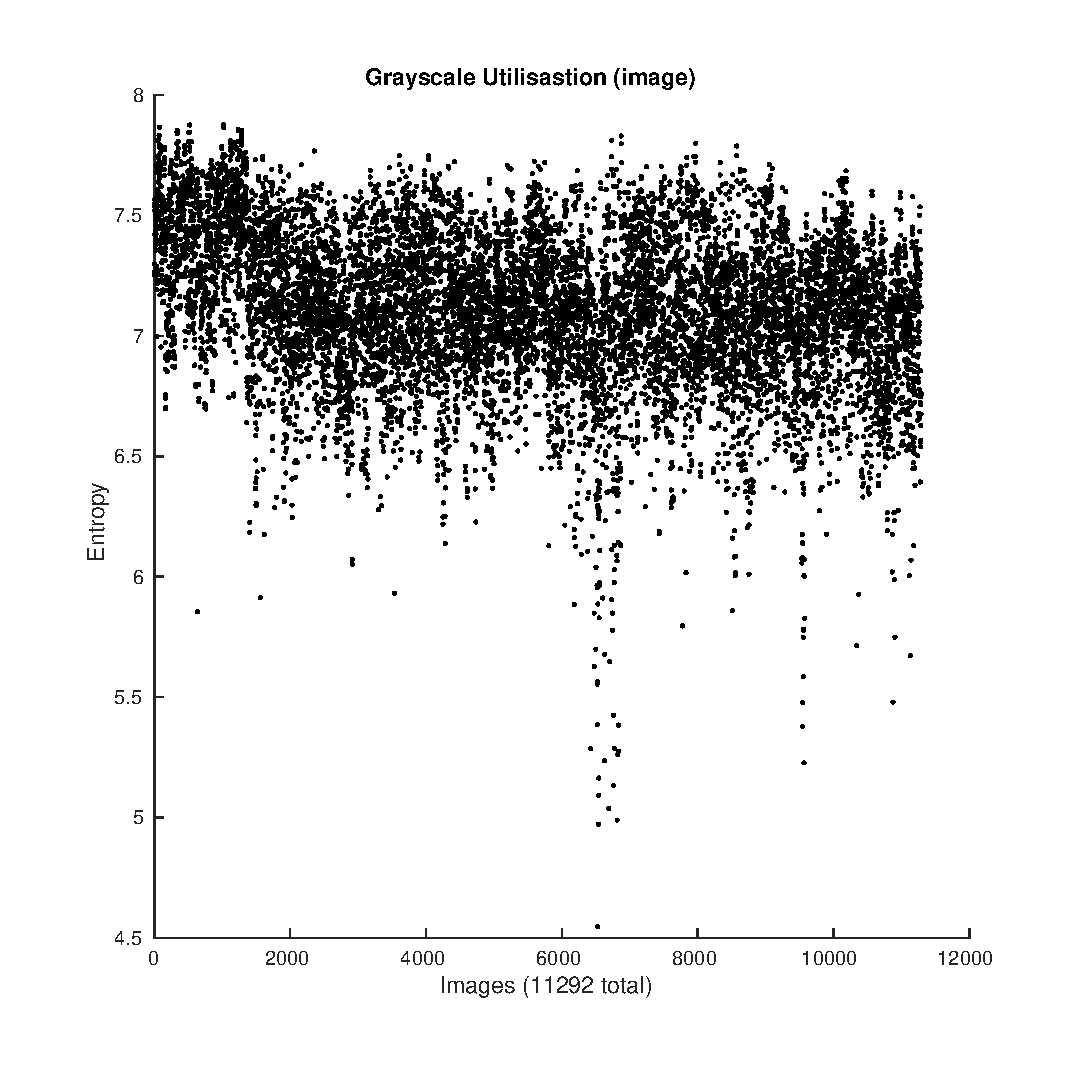
\includegraphics[height=2cm, width=5cm]{pics/biqa_dist_gsu_full}
		\caption{GSU of image \cite{iso}}
		\label{fig:gsuf}
	\end{wrapfigure}
As described in the previous sections GSU is calculated as the entropy of the
grey scale values that occur in a section or the entire image.  As seen in figure
\ref{fig:gsuf}, the distribution is equal to a normal distribution.  It also
shows that there are images with higher entropy than the rest, especially the
NTNU and MICHE data sets.  It also clearly shows images with lower entropy than
the rest.


\vspace{-5mm}
\subsubsection{BIQA - NIQE Metric}\vspace{-5mm}
	\begin{wrapfigure}{R}{0.325\linewidth}
		\centering
		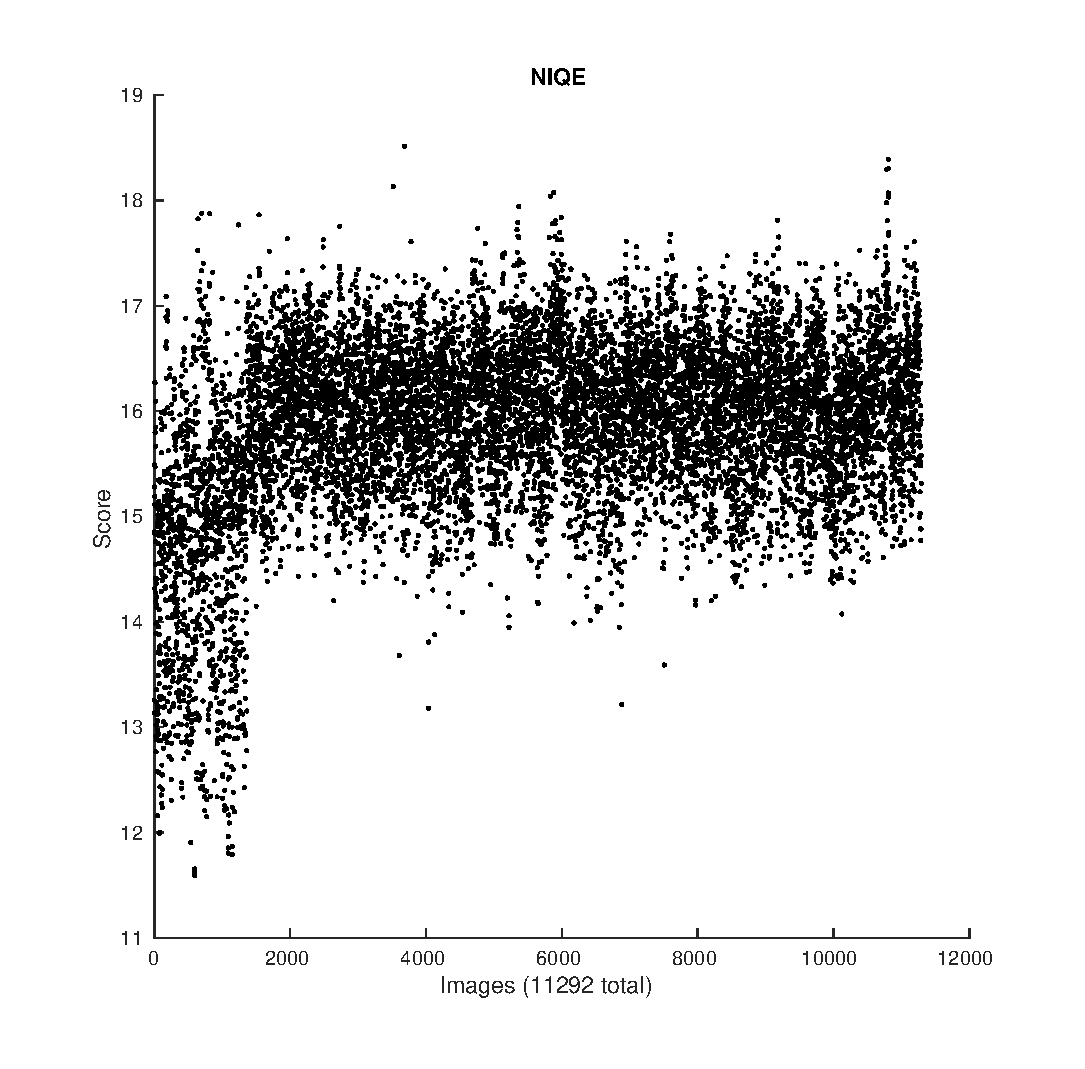
\includegraphics[height=2cm, width=5cm]{pics/biqa_dist_niqe}
		\caption{NIQE alg \cite{niqe}}
		\label{fig:niqe}
	\end{wrapfigure}
Anish Mittal et. al developed Natural Image Quality Evaluator (NIQE), a blind 
image quality model\cite{niqe}.  It assesses the image based on natural scene
statistics (NSS) as explained by L. Ruderman\cite{nss}.
In this model the resulting quality metric is described as the lower values
dictate better natural scene statistics. Therefore higher quality value is
related to a lower output value from NIQE.

Given this statistic, a method for performing classification should be very
possible, but as seen in figure \ref{fig:niqe} a distinct singular value
separating the system does not appear directly.  However one can see that there
are a quite normal distribution where the outliers represent certain images that
are of much higher quality and lower quality.


\vspace{-5mm}
\subsubsection{BIQA - BRISQUE Metric}\vspace{-5mm}
	\begin{wrapfigure}{R}{0.325\linewidth}
		\centering
		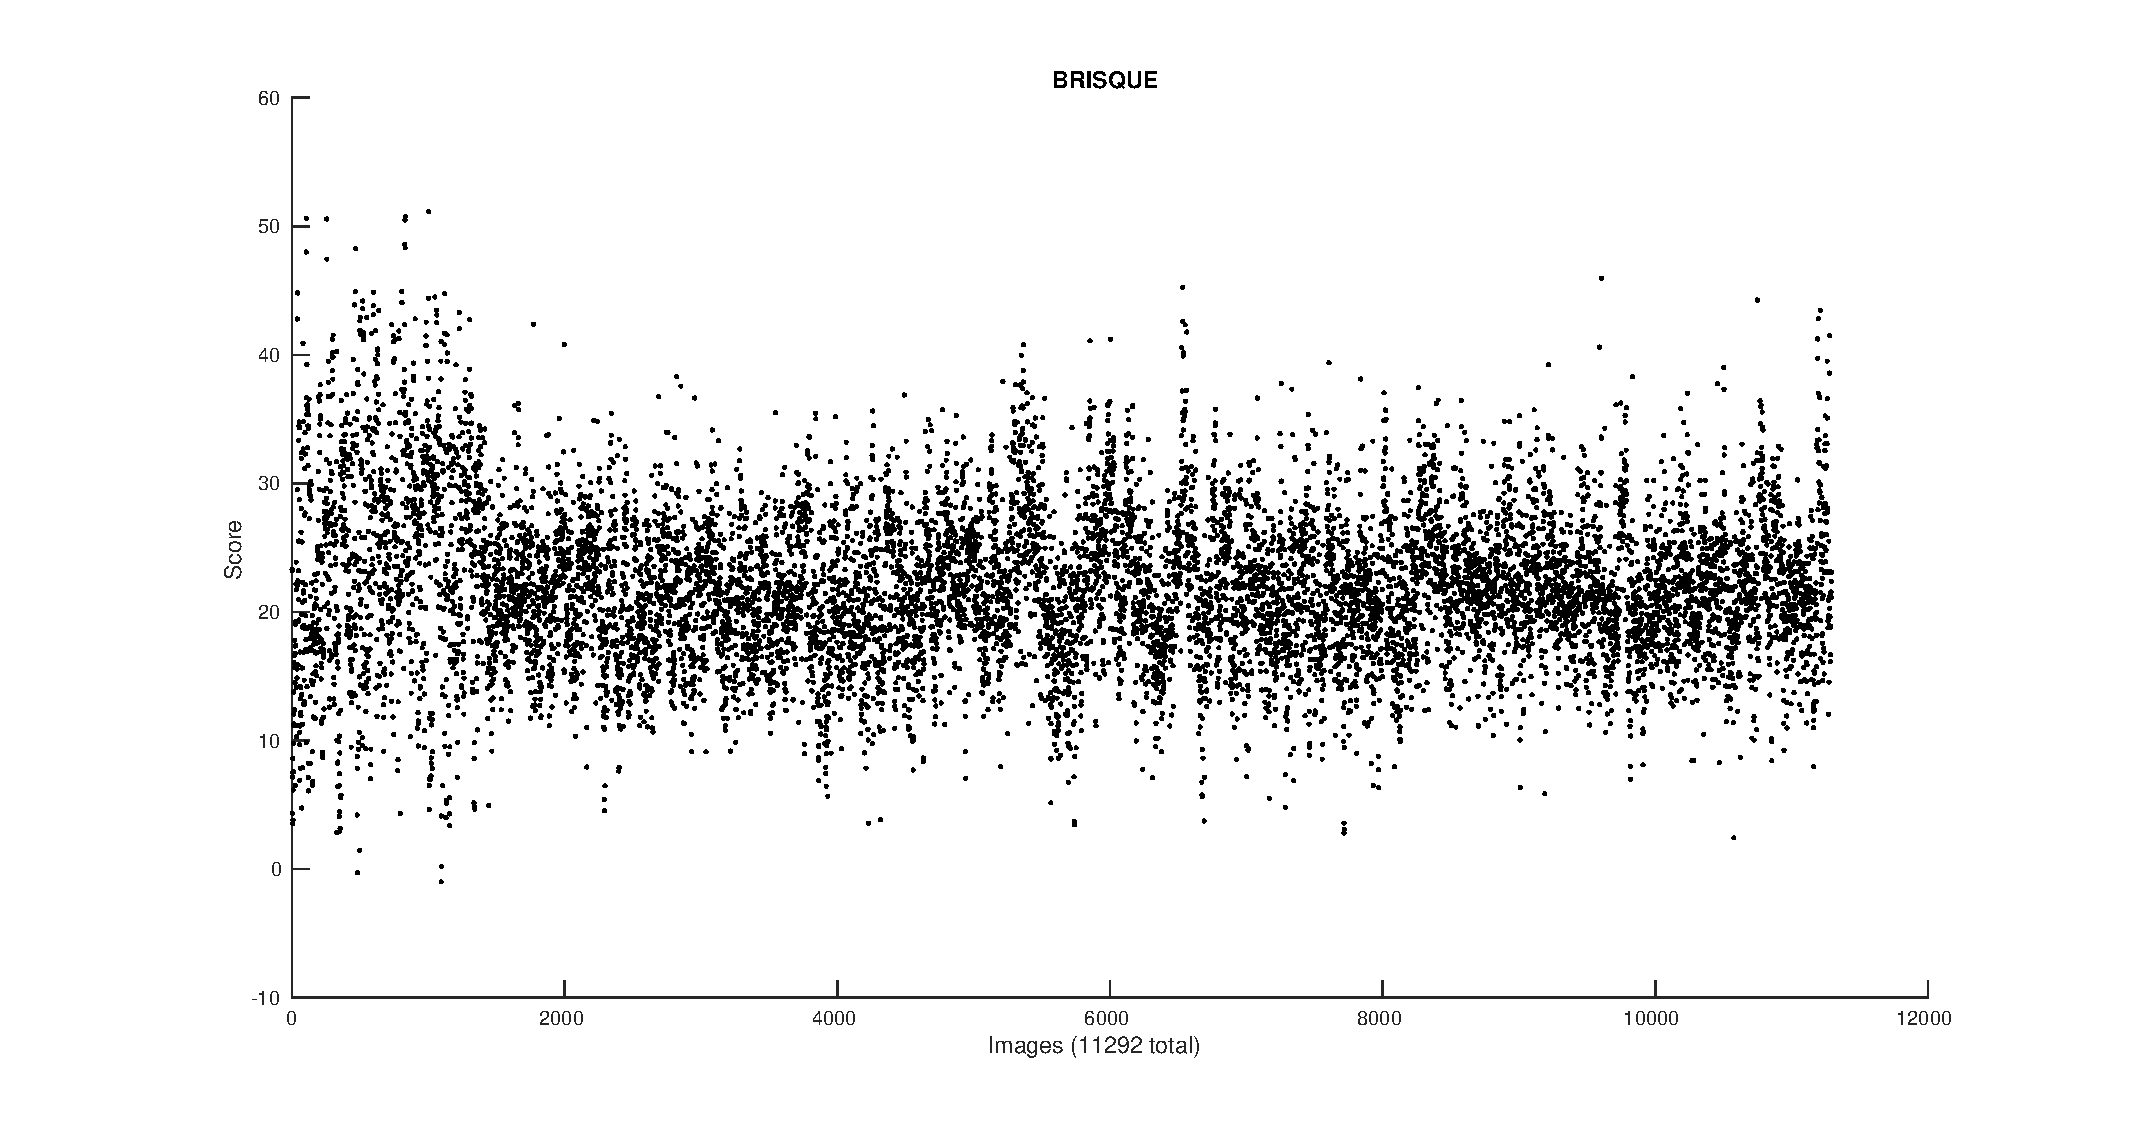
\includegraphics[height=2.25cm, width=5cm]{pics/biqa_dist_brisque}
		\caption{BRISQUE alg \cite{brisque}}
		\label{fig:brisque}
	\end{wrapfigure}
The BRISQUE metric is calculated by the tool developed by Anish Mittal et.
al\cite{brisque}. They have developed a blind image quality assessment model
operating in the spacial domain.  As with NIQE, BRISQUE also focuses on the use
of scene statistics to quantify the quality.  It evaluates the possible loss of
"naturalness".
As with many of the others metrics, there is a clear normal distribution as
well. Images that are of better quality, has a lower metric value than those of
inferior quality.


\vspace{-5mm}
\subsubsection{BIQA - JP2KNR Metric}\vspace{-5mm}
	\begin{wrapfigure}{R}{0.325\linewidth}
		\centering
		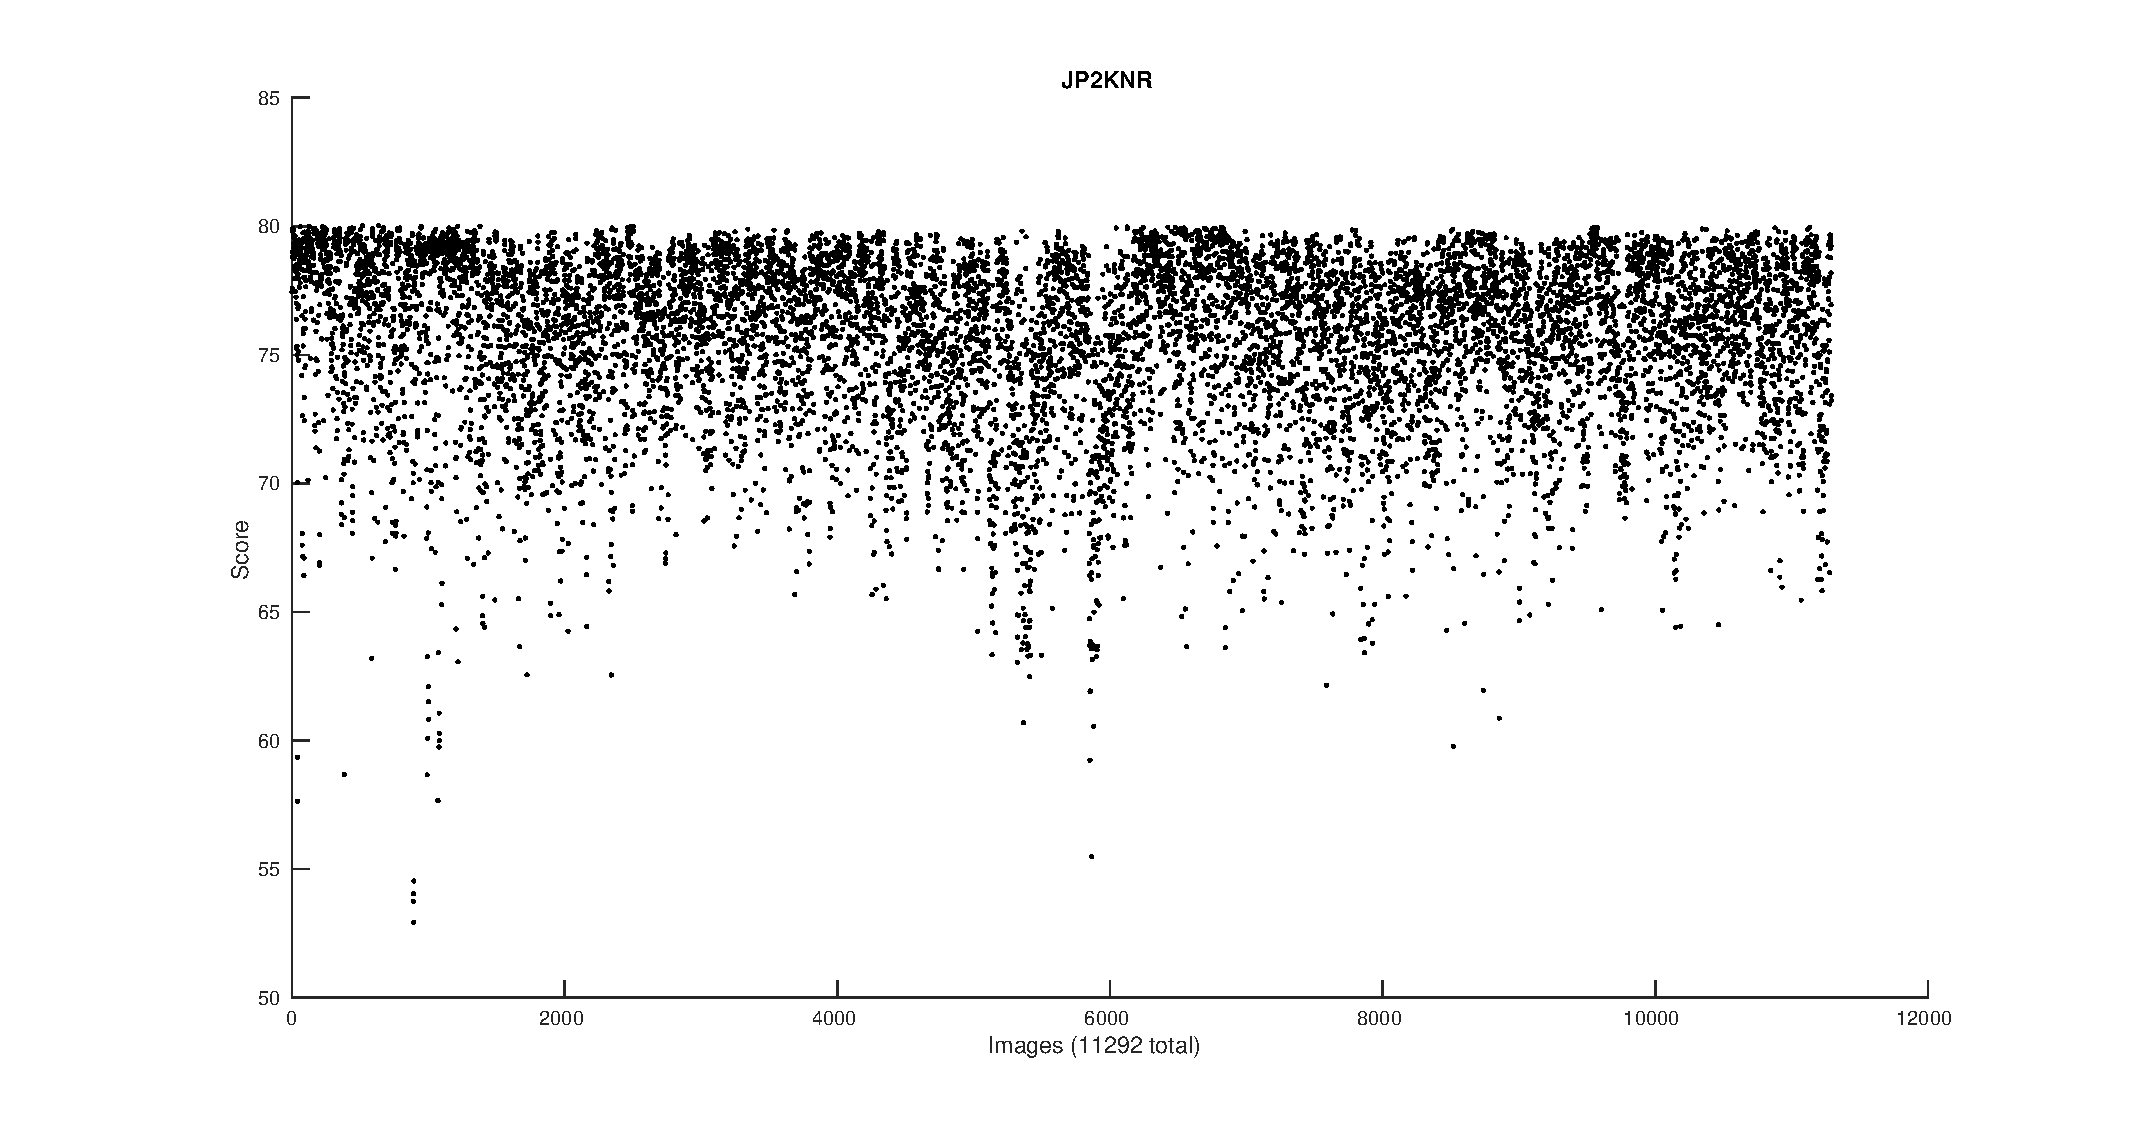
\includegraphics[height=2.75cm, width=5cm]{pics/biqa_dist_jp2knr}
		\caption{JP2KNR alg \cite{jp2knr}}
		\label{fig:jp2knr}
	\end{wrapfigure}
Hamid R. Sheikh et. al created the JP2KNR tool, which employs a method of
applying natural scene statistics to measure quality of images that has been
compressed using wavelet compression.  It seeks to quantify the the loss of
quality which can be related to the human perception of quality.
As opposed to BRISQUE and NIQE, JP2KNRs metric value states that a higher value
is equal to higher quality and low metric value is equal to a lower metric
value.
As shown in figure \ref{fig:jp2knr}, there is a distinct value of the images
with a quite clear maximum level of quality.  This gives the distribution of a
peak positioned to the far right-side of the graph.


\vspace{-5mm}
\subsubsection{BIQA - BIQI Metric}\vspace{-5mm}
	\begin{wrapfigure}{R}{0.325\linewidth}
		\centering
		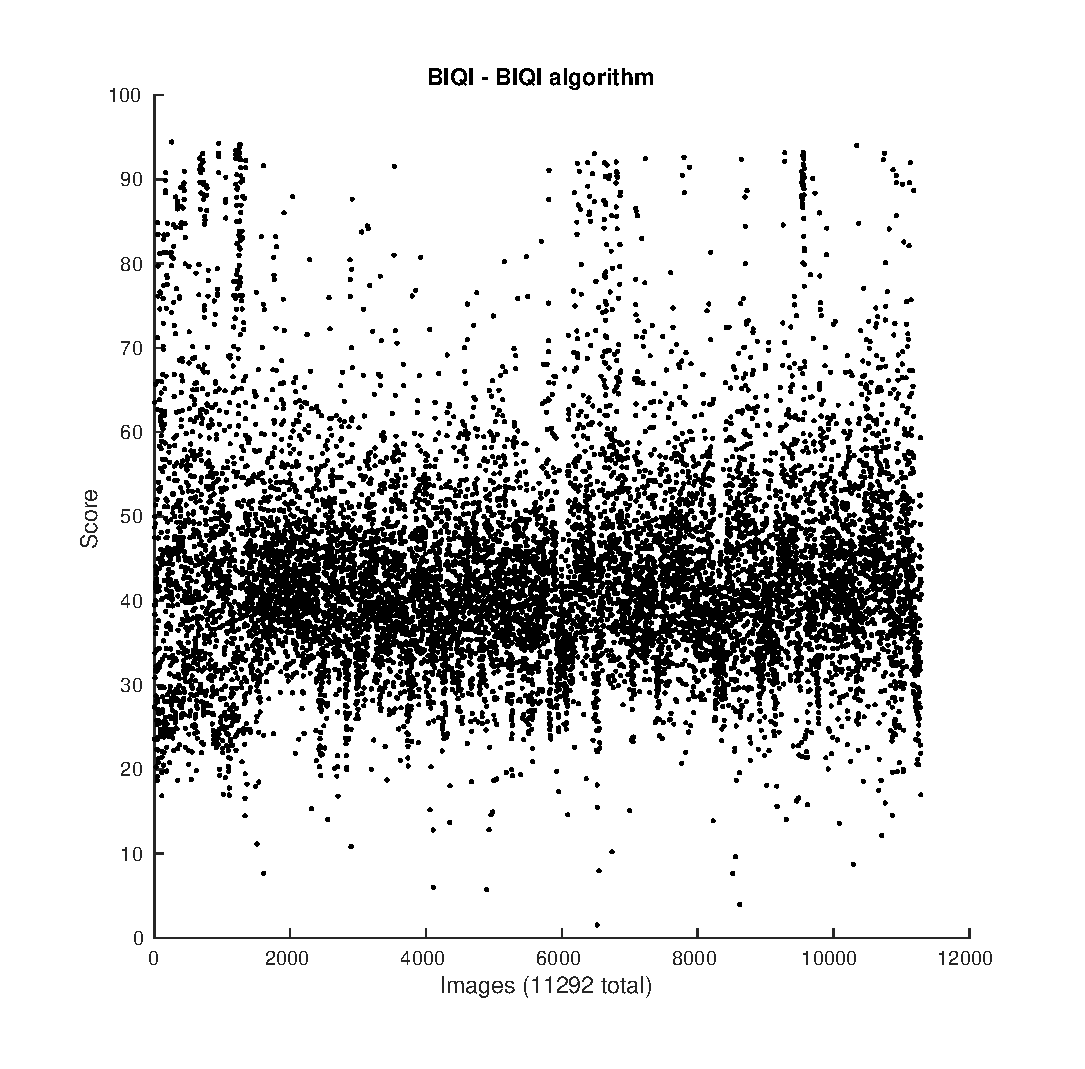
\includegraphics[height=2.75cm, width=5cm]{pics/biqa_dist_biqi_alg}
		\caption{BIQI alg \cite{biqi}}
		\label{fig:biqialg}
	\end{wrapfigure}
"Blind Image Quality Index", BIQI\cite{biqi} was developed by Anush K. Moorthy
et. al and focused on assessing the distortions of the image.  BIQI is based on
a pre-trained classifier that can be used to assess any distortion, and it is
also based on NSS.
The distribution is not as clear as with many of the other data sets, but has a
centralised distribution between 35-50 for the UBIRISv2 data set. The NTNU and
MICHE data sets does not seem to have any centralised distribution.
BIQI may therefore be unsuitable for classification.


\subsection{Classification}
After performing the classification on each of the selected metrics separately,
several of them where shown to be unable to classify the images evenly.  Even
though the training set was slightly overfitted for "good" images.

As one can see several of the metrics performed poorly, either classifying
falsely or not at all.  The IQA pupil dilation metric (fig. \ref{fig:clas_pd}),
IQA iris area (fig. \ref{fig:clas_ia}), IQA usable iris (fig. \ref{fig:clas_ua})
IQA focus assessment (fig. \ref{fig:clas_f}) and IQA motion magnitude metric
(fig. \ref{fig:clas_mot}), performed very poorly.  The pupil dilation metric are
unable to classify any as "good", while usable iris area, classifies them
with 0\%\ as "good images", and iris area classifies a few as "good".

Table \ref{tab:indclas} summarises the number classification made by the support
vector machine (SVM) after being trained with 625 "good" images and 560 "bad"
images which was manually classified with WebIIC\cite{webiic}.

\begin{figure}[h]
	\begin{minipage}{0.48\linewidth}
		\centering
		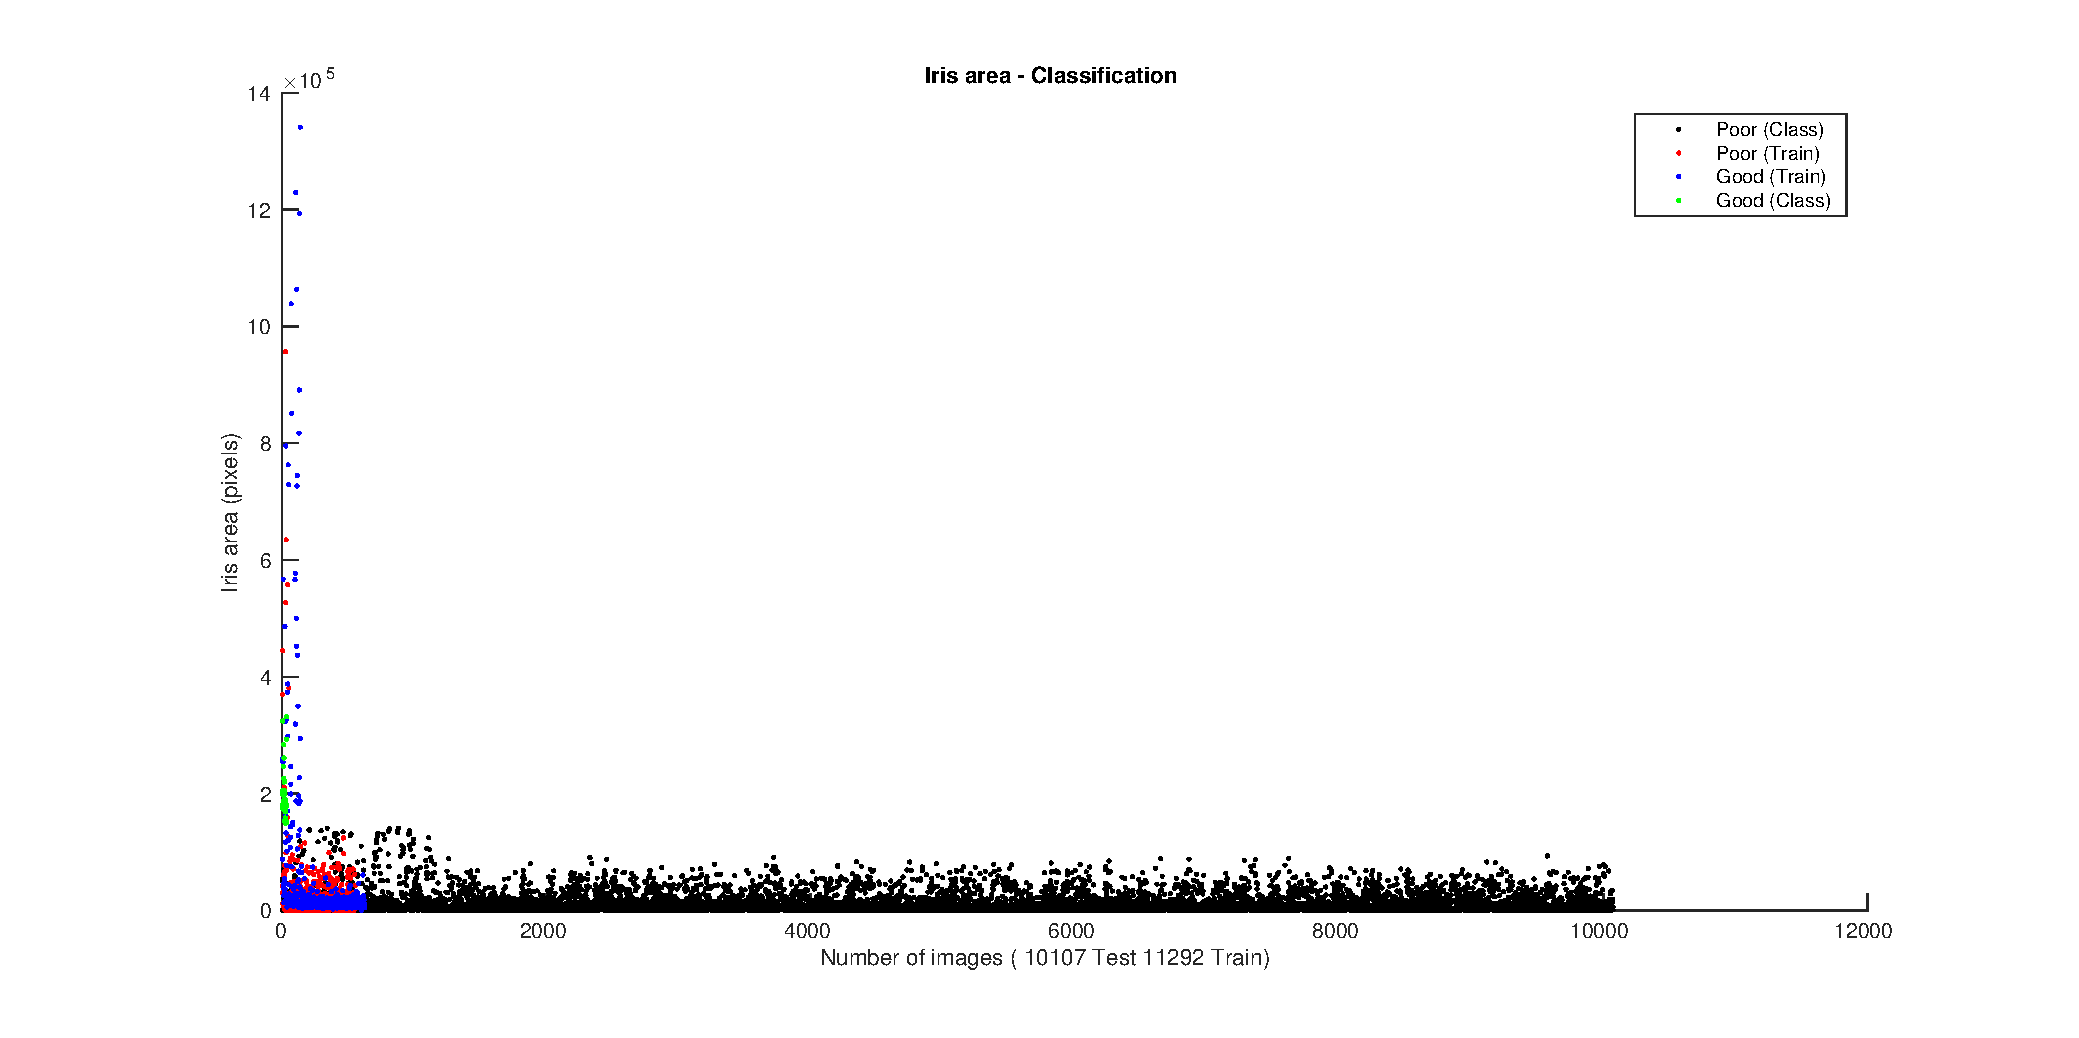
\includegraphics[width=0.9\linewidth, height=1.6cm]{pics/iqa_clas_area}
		\caption{Res. of class. using IQA iris area}
		\label{fig:clas_ia}
	\end{minipage}
	\hfill
	\begin{minipage}{0.48\linewidth}
		\centering
		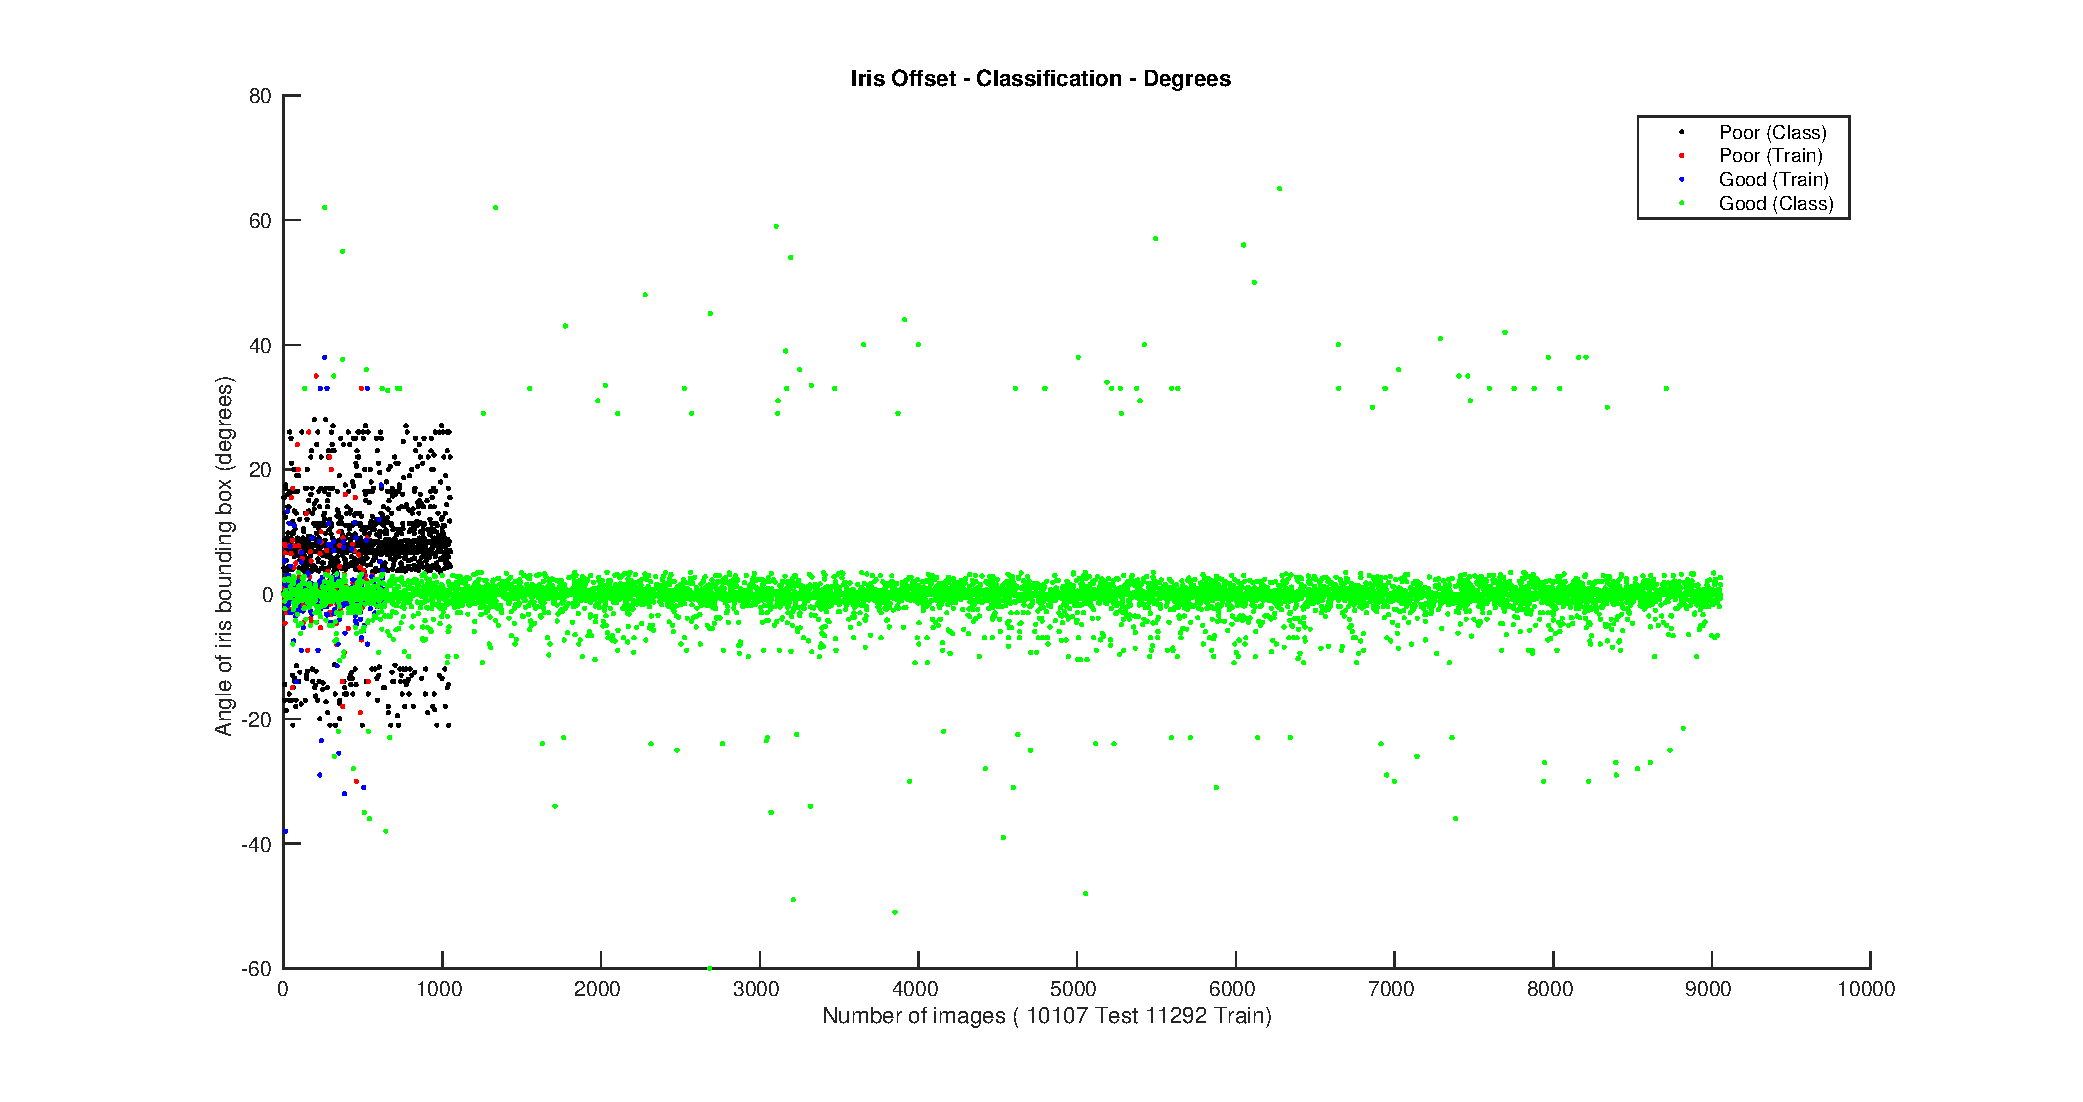
\includegraphics[width=0.9\linewidth, height=1.6cm]{pics/iqa_clas_iris_angle}
		\caption{Res. of class. using IQA iris angle}
		\label{fig:clas_ang}
	\end{minipage}
	\begin{minipage}{0.48\linewidth}
		\centering
		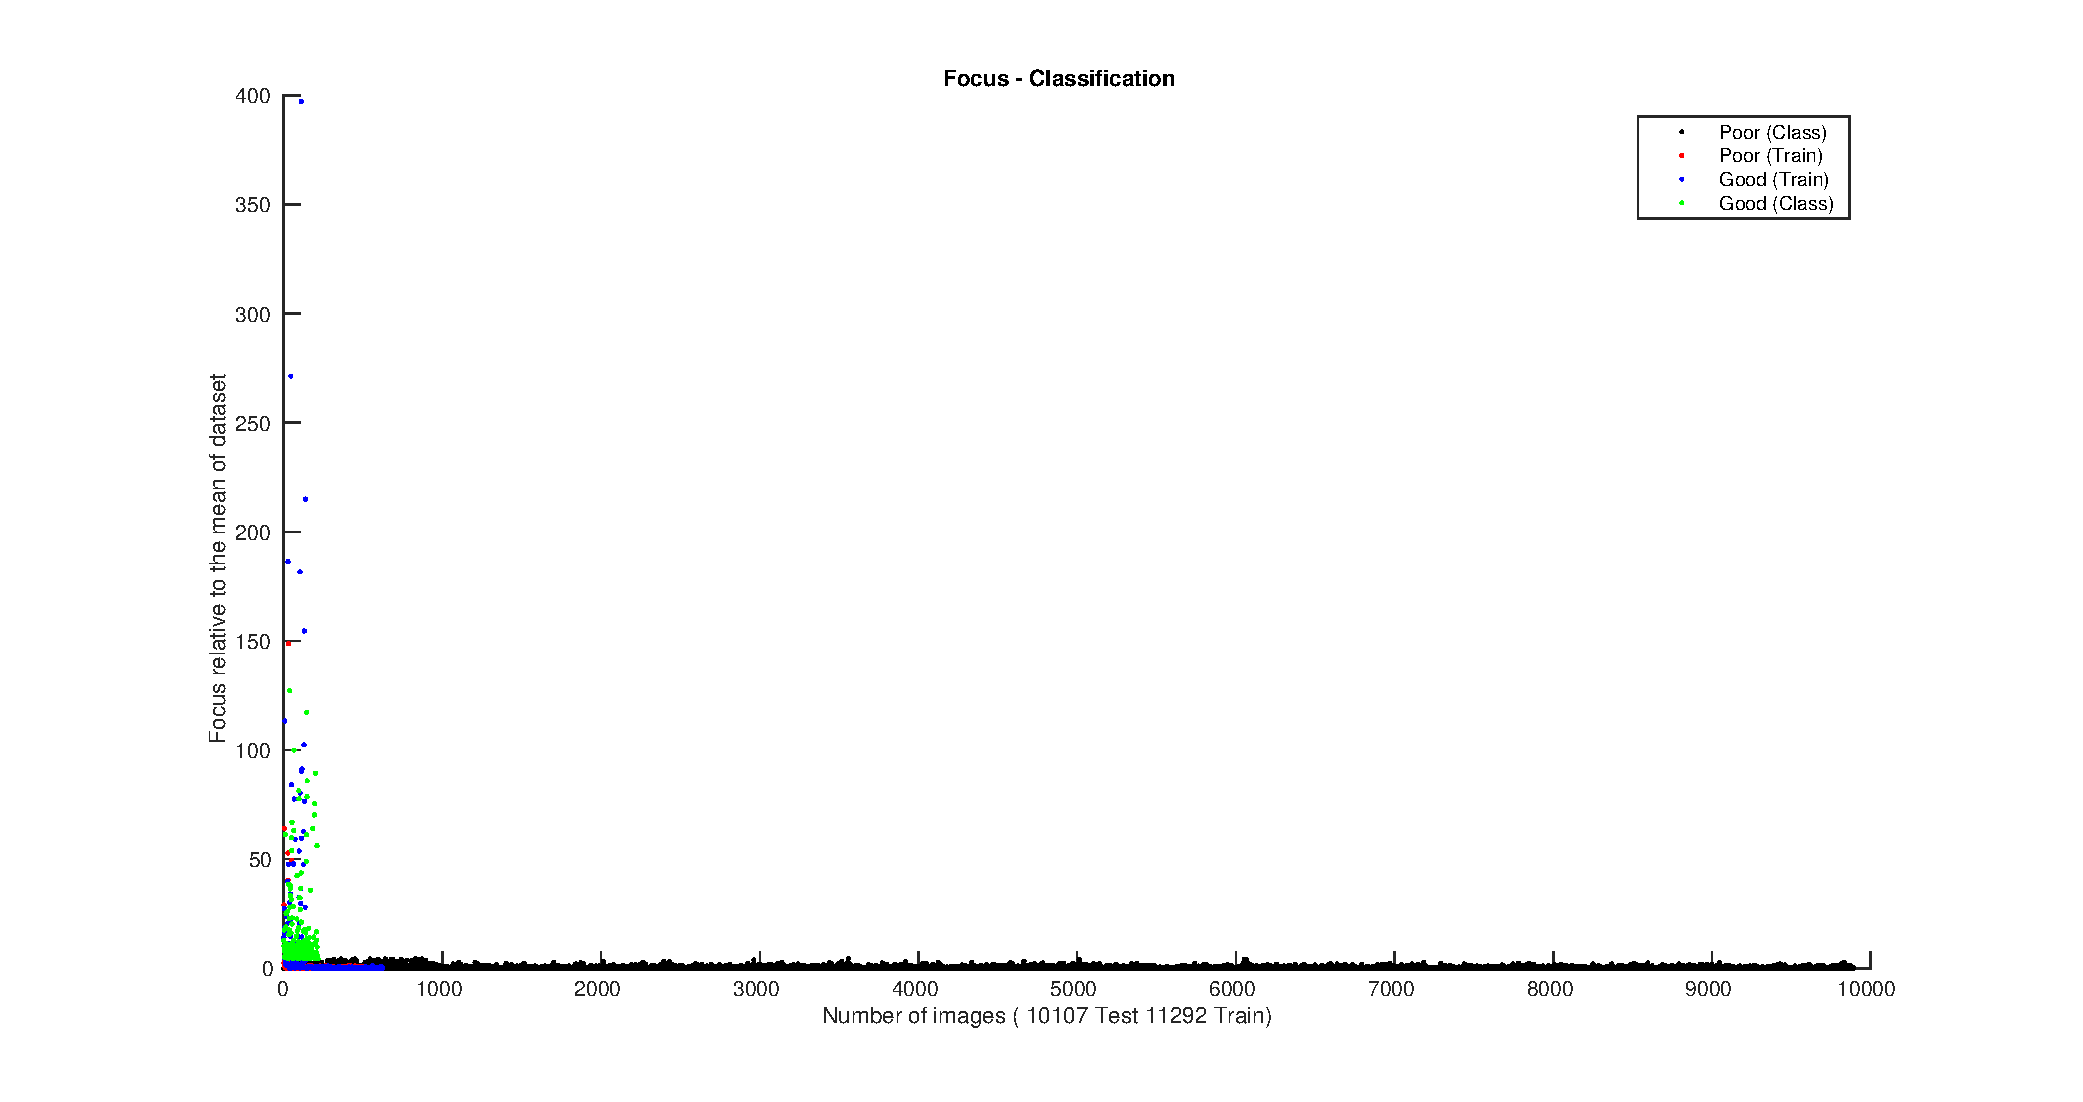
\includegraphics[width=0.9\linewidth, height=1.6cm]{pics/iqa_clas_focus}
		\caption{Res. of class. using IQA focus}
		\label{fig:clas_f}
	\end{minipage}
	\hfill
	\begin{minipage}{0.48\linewidth}
		\centering
		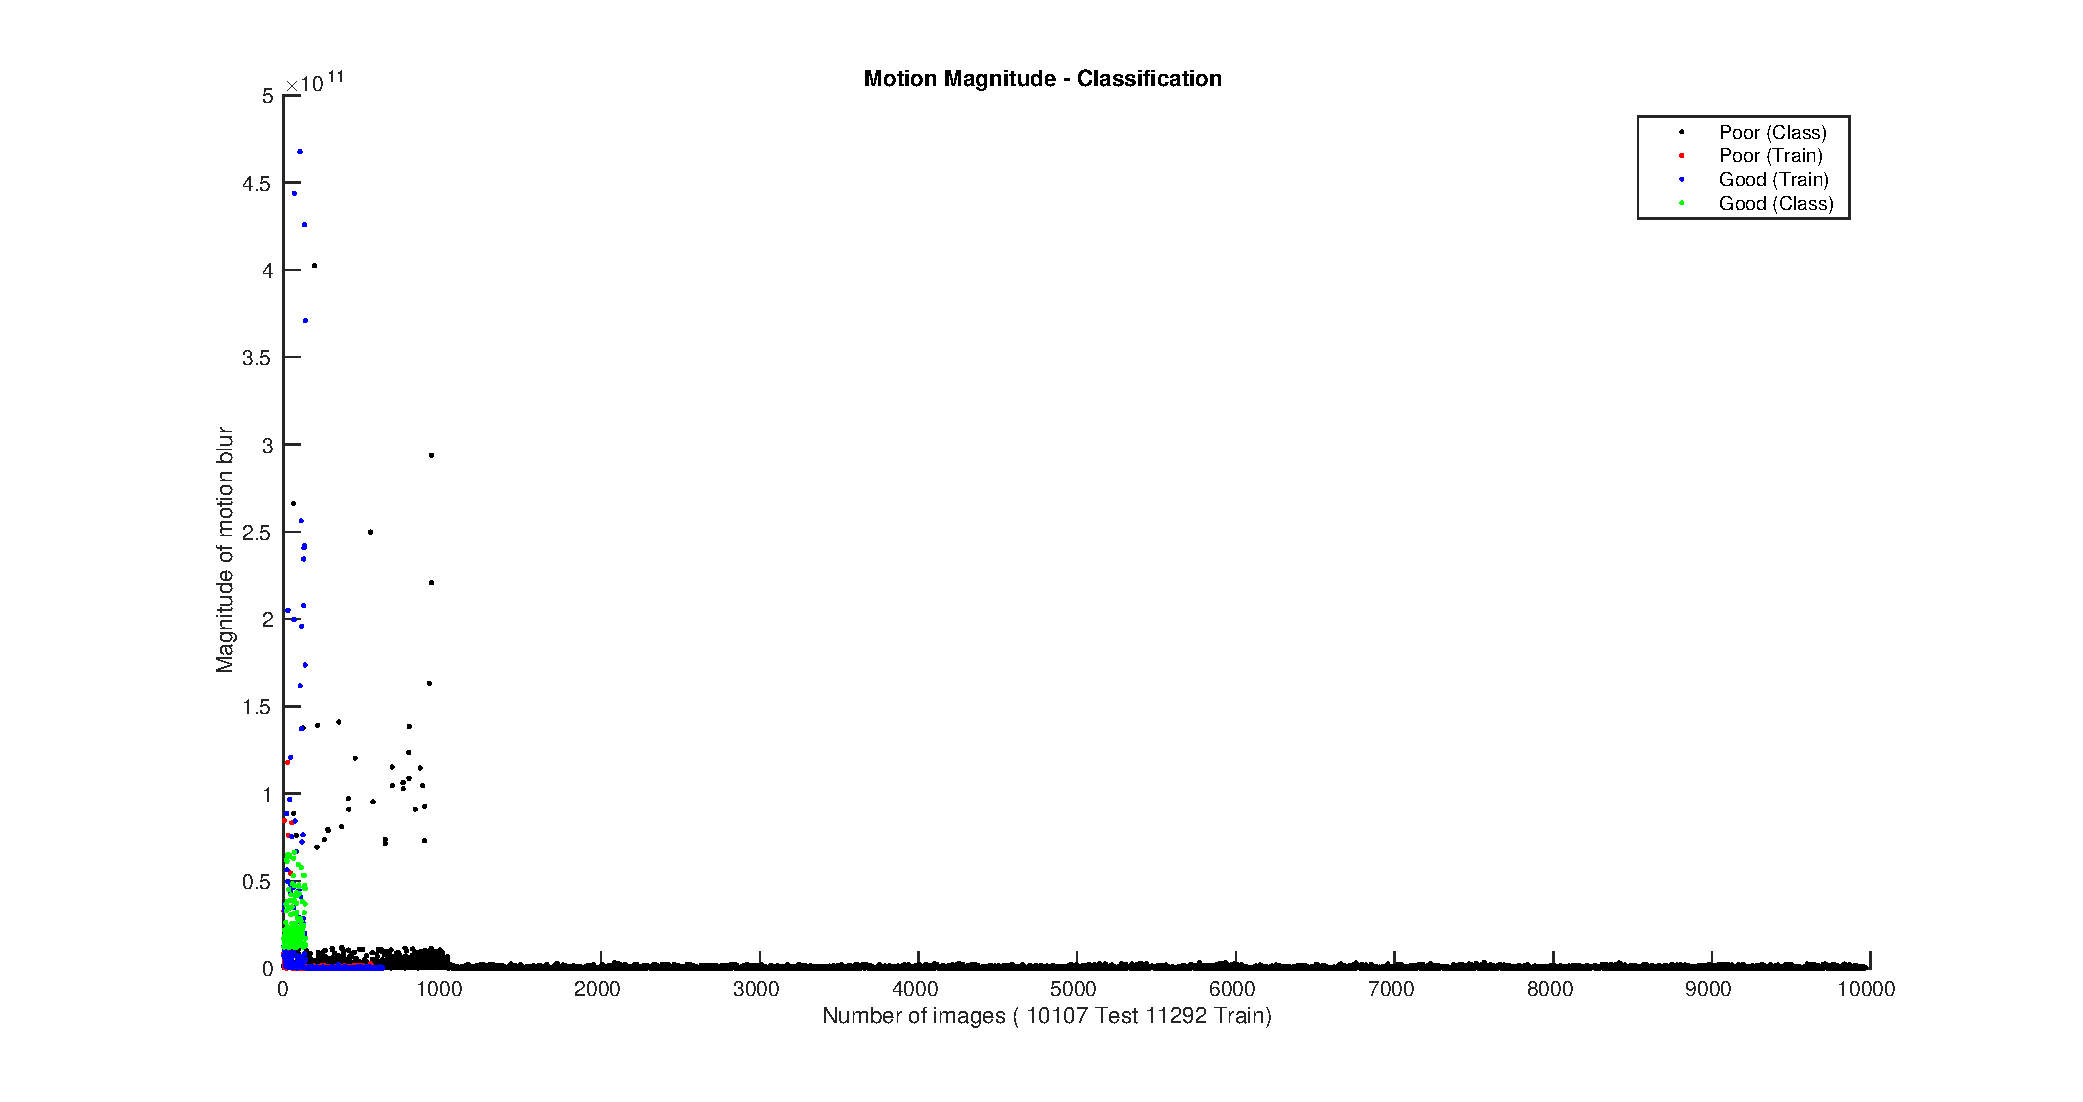
\includegraphics[width=0.9\linewidth, height=1.6cm]{pics/iqa_clas_motion}
		\caption{Res. of class. using IQA motion}
		\label{fig:clas_mot}
	\end{minipage}
	\begin{minipage}{0.48\linewidth}
		\centering
		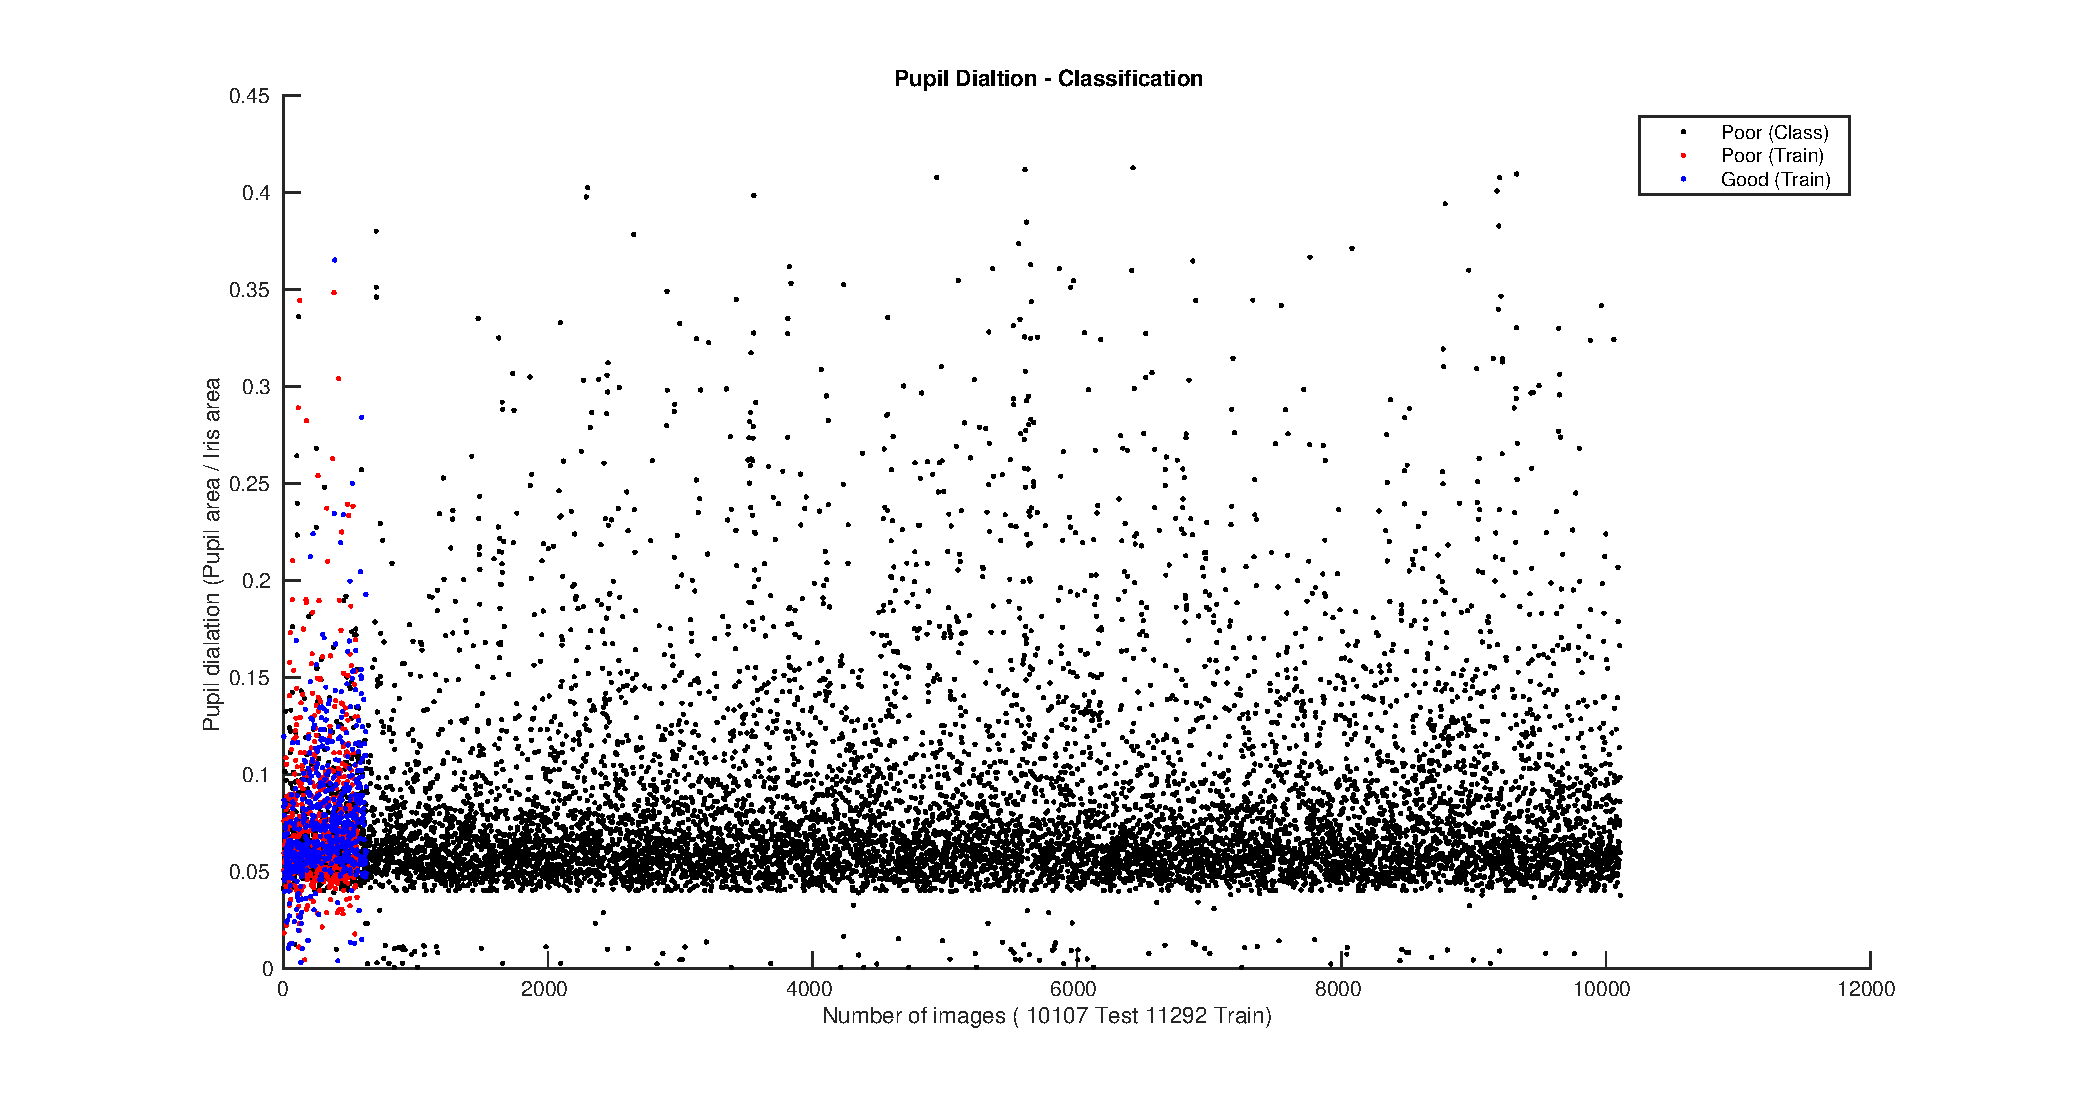
\includegraphics[width=0.9\linewidth, height=1.6cm]{pics/iqa_clas_pup_dial}
		\caption{Res. of class. using IQA pupil dilation}
		\label{fig:clas_pd}
	\end{minipage}
	\hfill
	\begin{minipage}{0.48\linewidth}
		\centering
		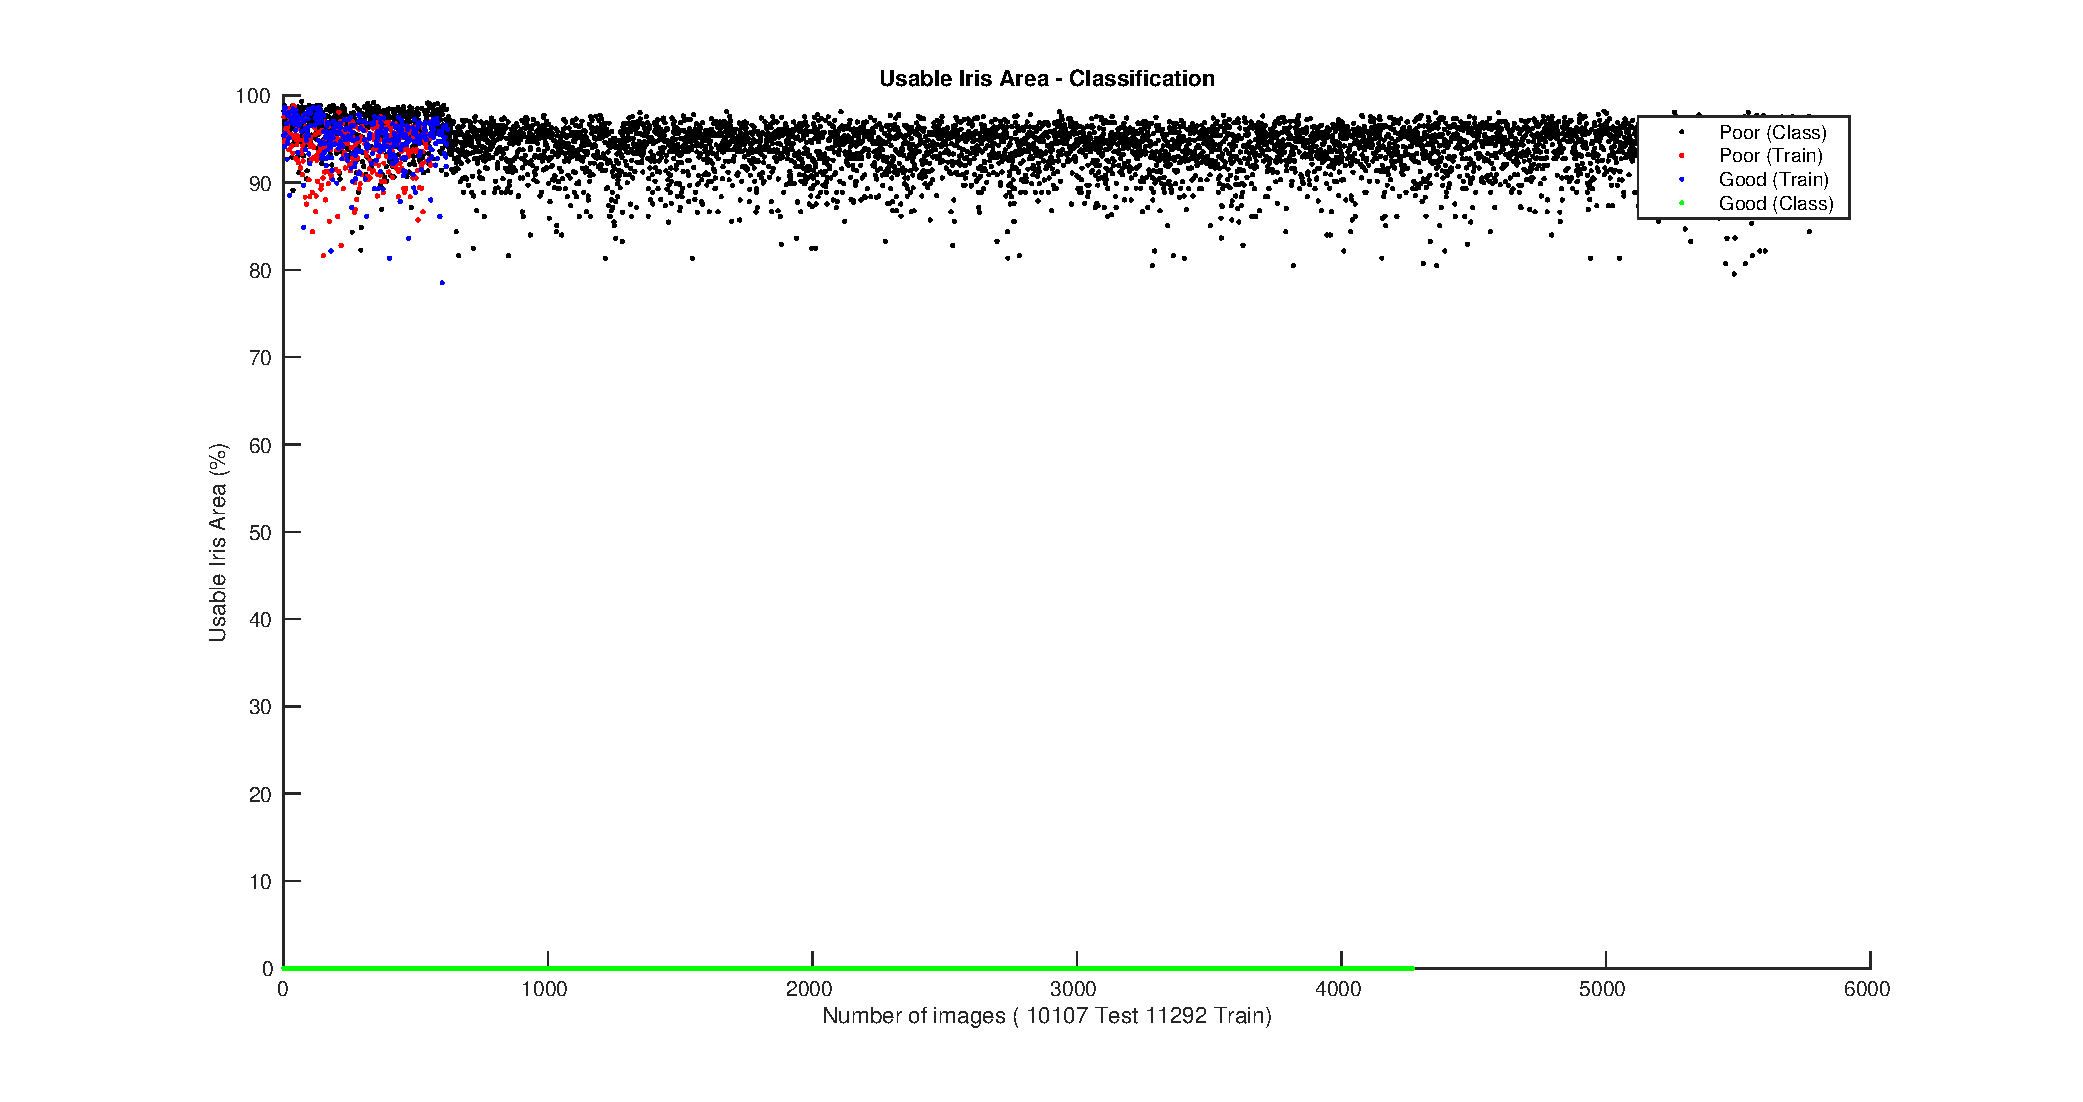
\includegraphics[width=0.9\linewidth, height=1.6cm]{pics/iqa_clas_usable_area}
		\caption{Res. of class. using BIQA UIA}
		\label{fig:clas_ua}
	\end{minipage}
	\begin{minipage}{0.48\linewidth}
		\centering
		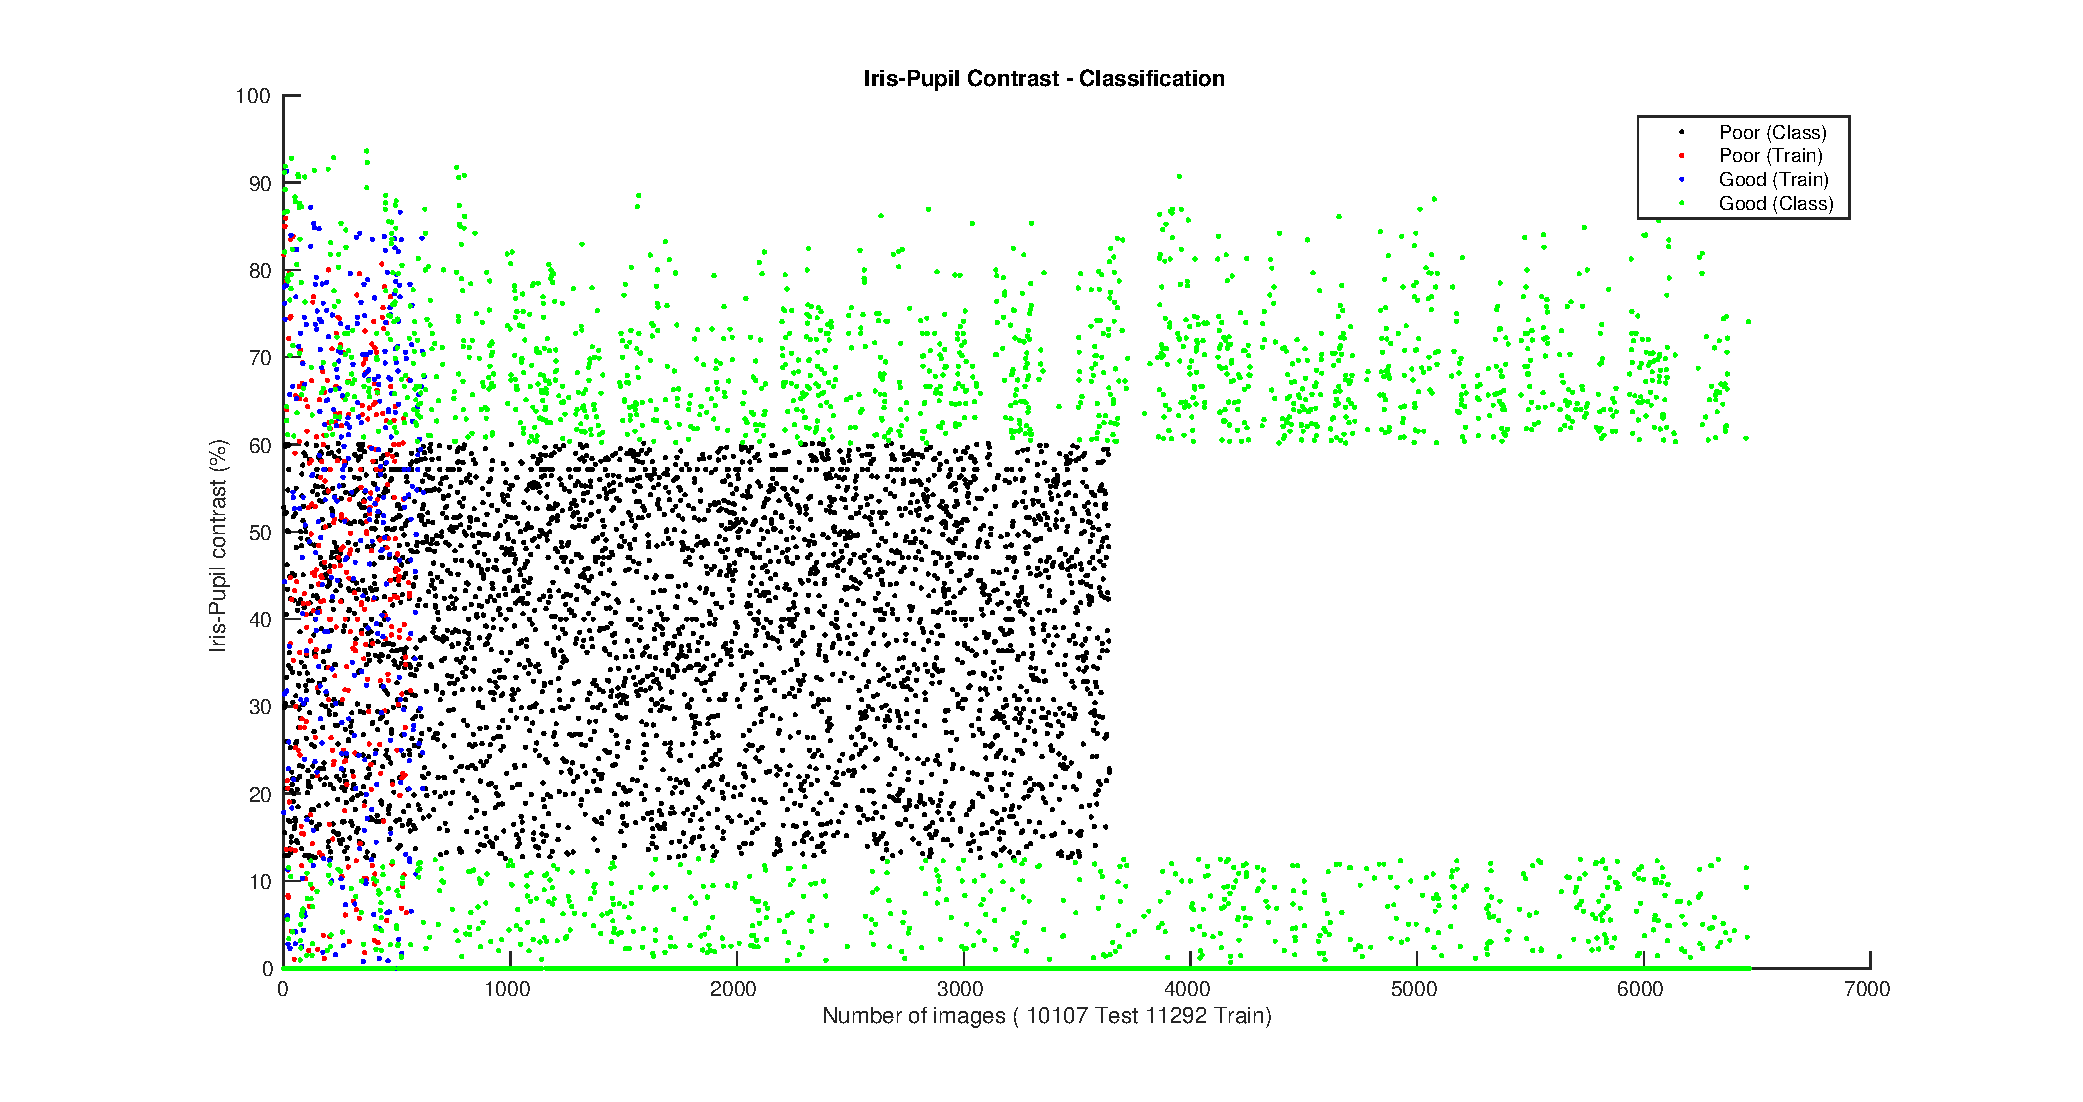
\includegraphics[width=0.9\linewidth, height=1.6cm]{pics/biqa_clas_ipc}
		\caption{Res. of class. using BIQA IPC}
		\label{fig:clas_ipc}
	\end{minipage}
	\hfill
	\begin{minipage}{0.48\linewidth}
		\centering
		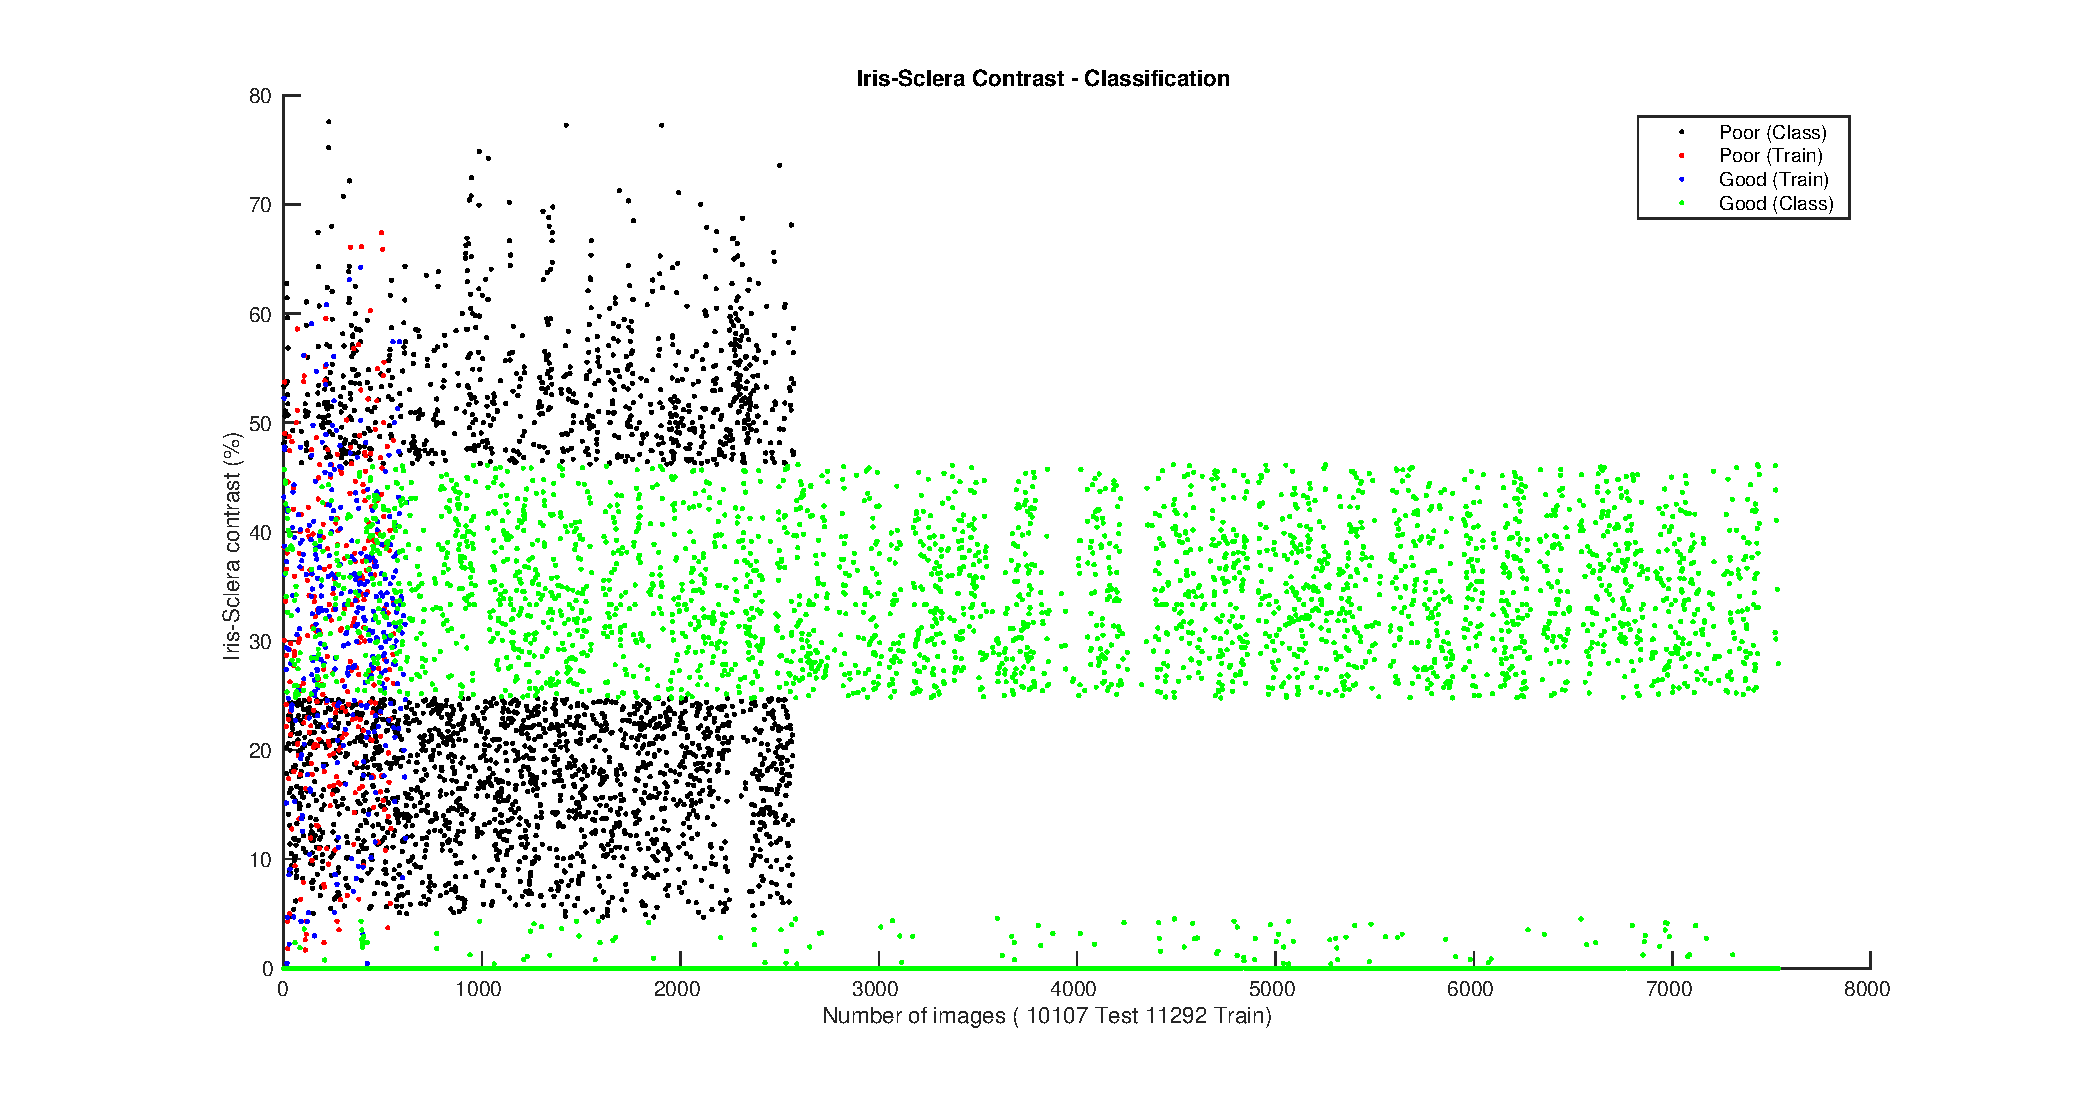
\includegraphics[width=0.9\linewidth, height=1.6cm]{pics/biqa_clas_isc}
		\caption{Res. of class. using BIQA ISC}
		\label{fig:clas_isc}
	\end{minipage}
	\begin{minipage}{0.48\linewidth}
		\centering
		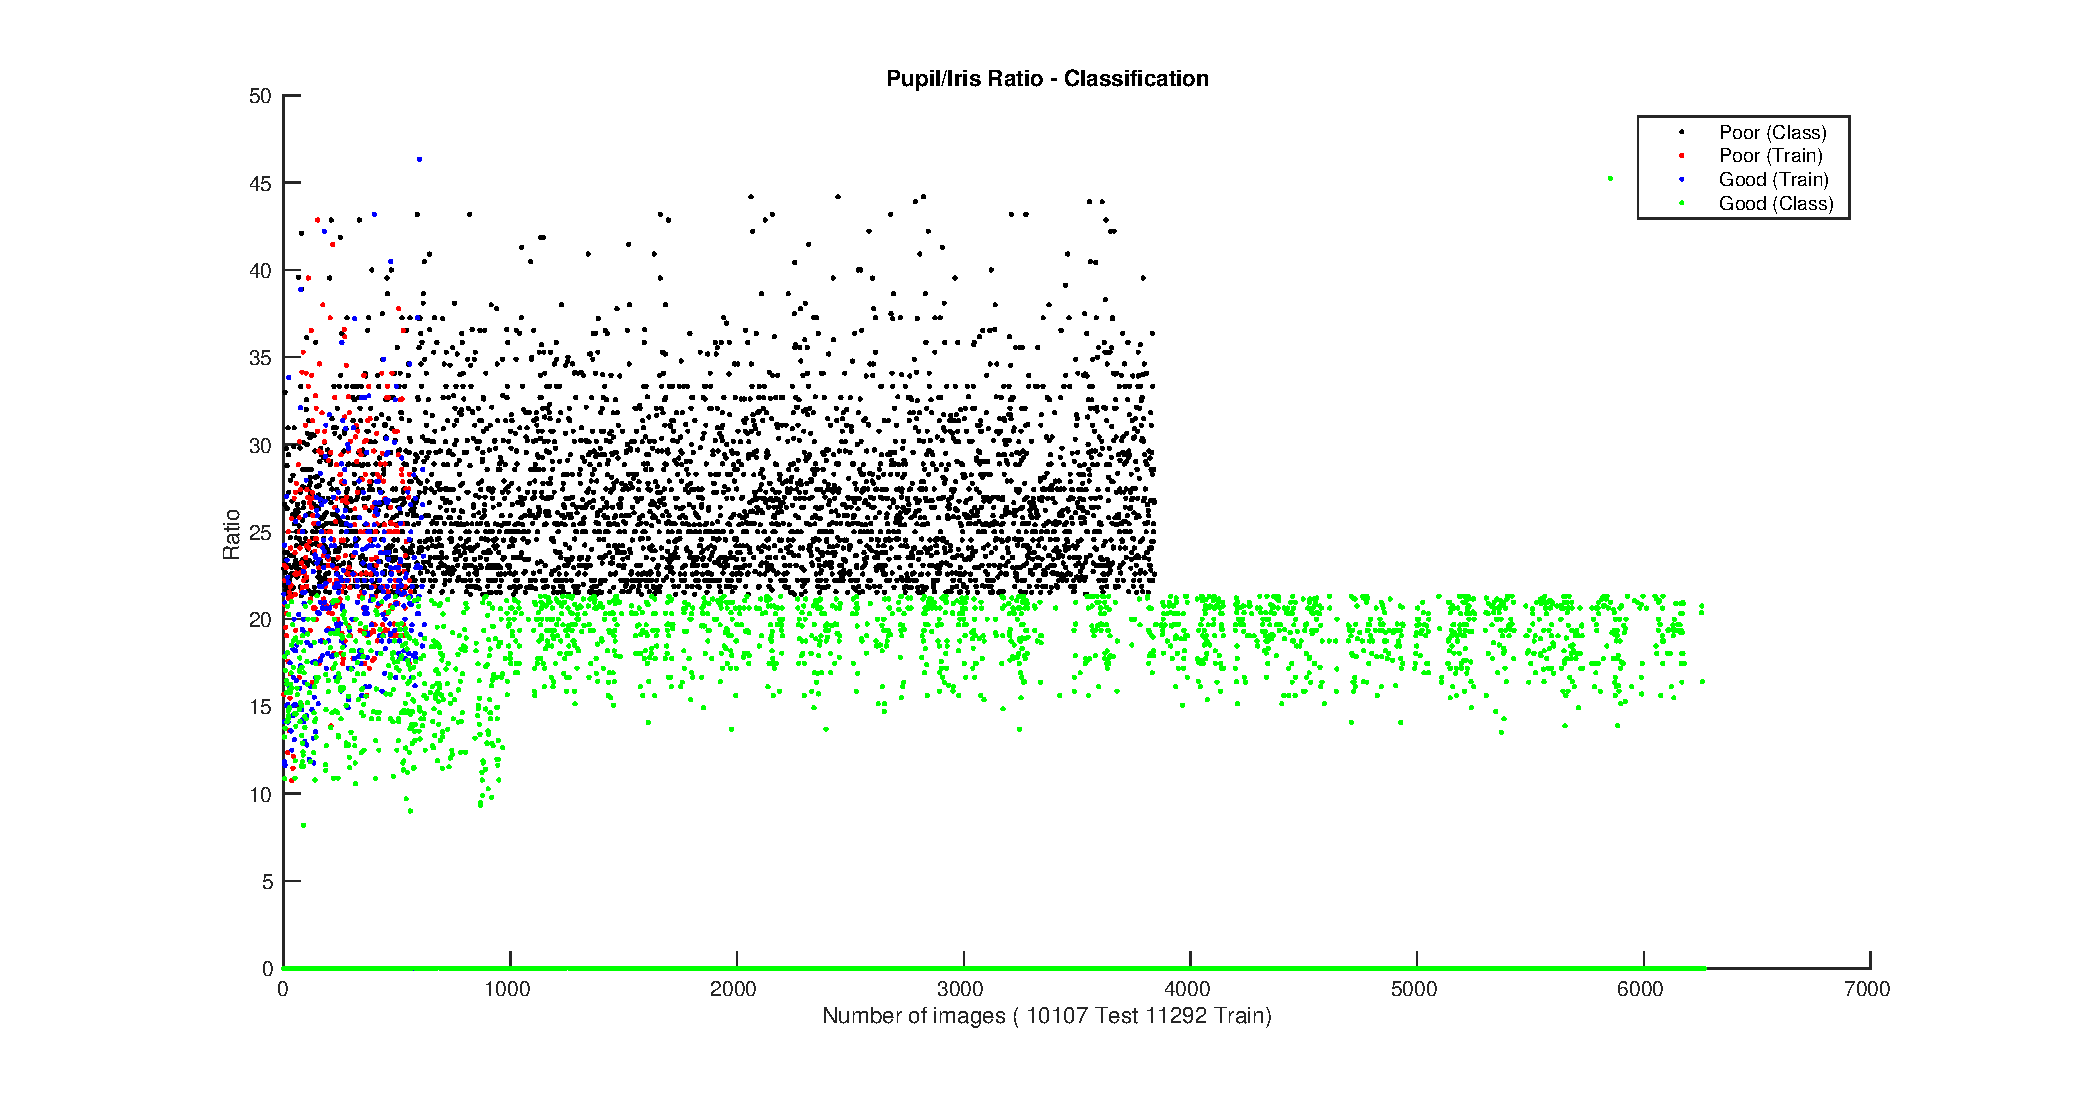
\includegraphics[width=0.9\linewidth, height=1.6cm]{pics/biqa_clas_pir}
		\caption{Res. of class. using BIQA pupil-iris rat.}
		\label{fig:clas_pir}
	\end{minipage}
	\hfill
	\begin{minipage}{0.48\linewidth}
		\centering
		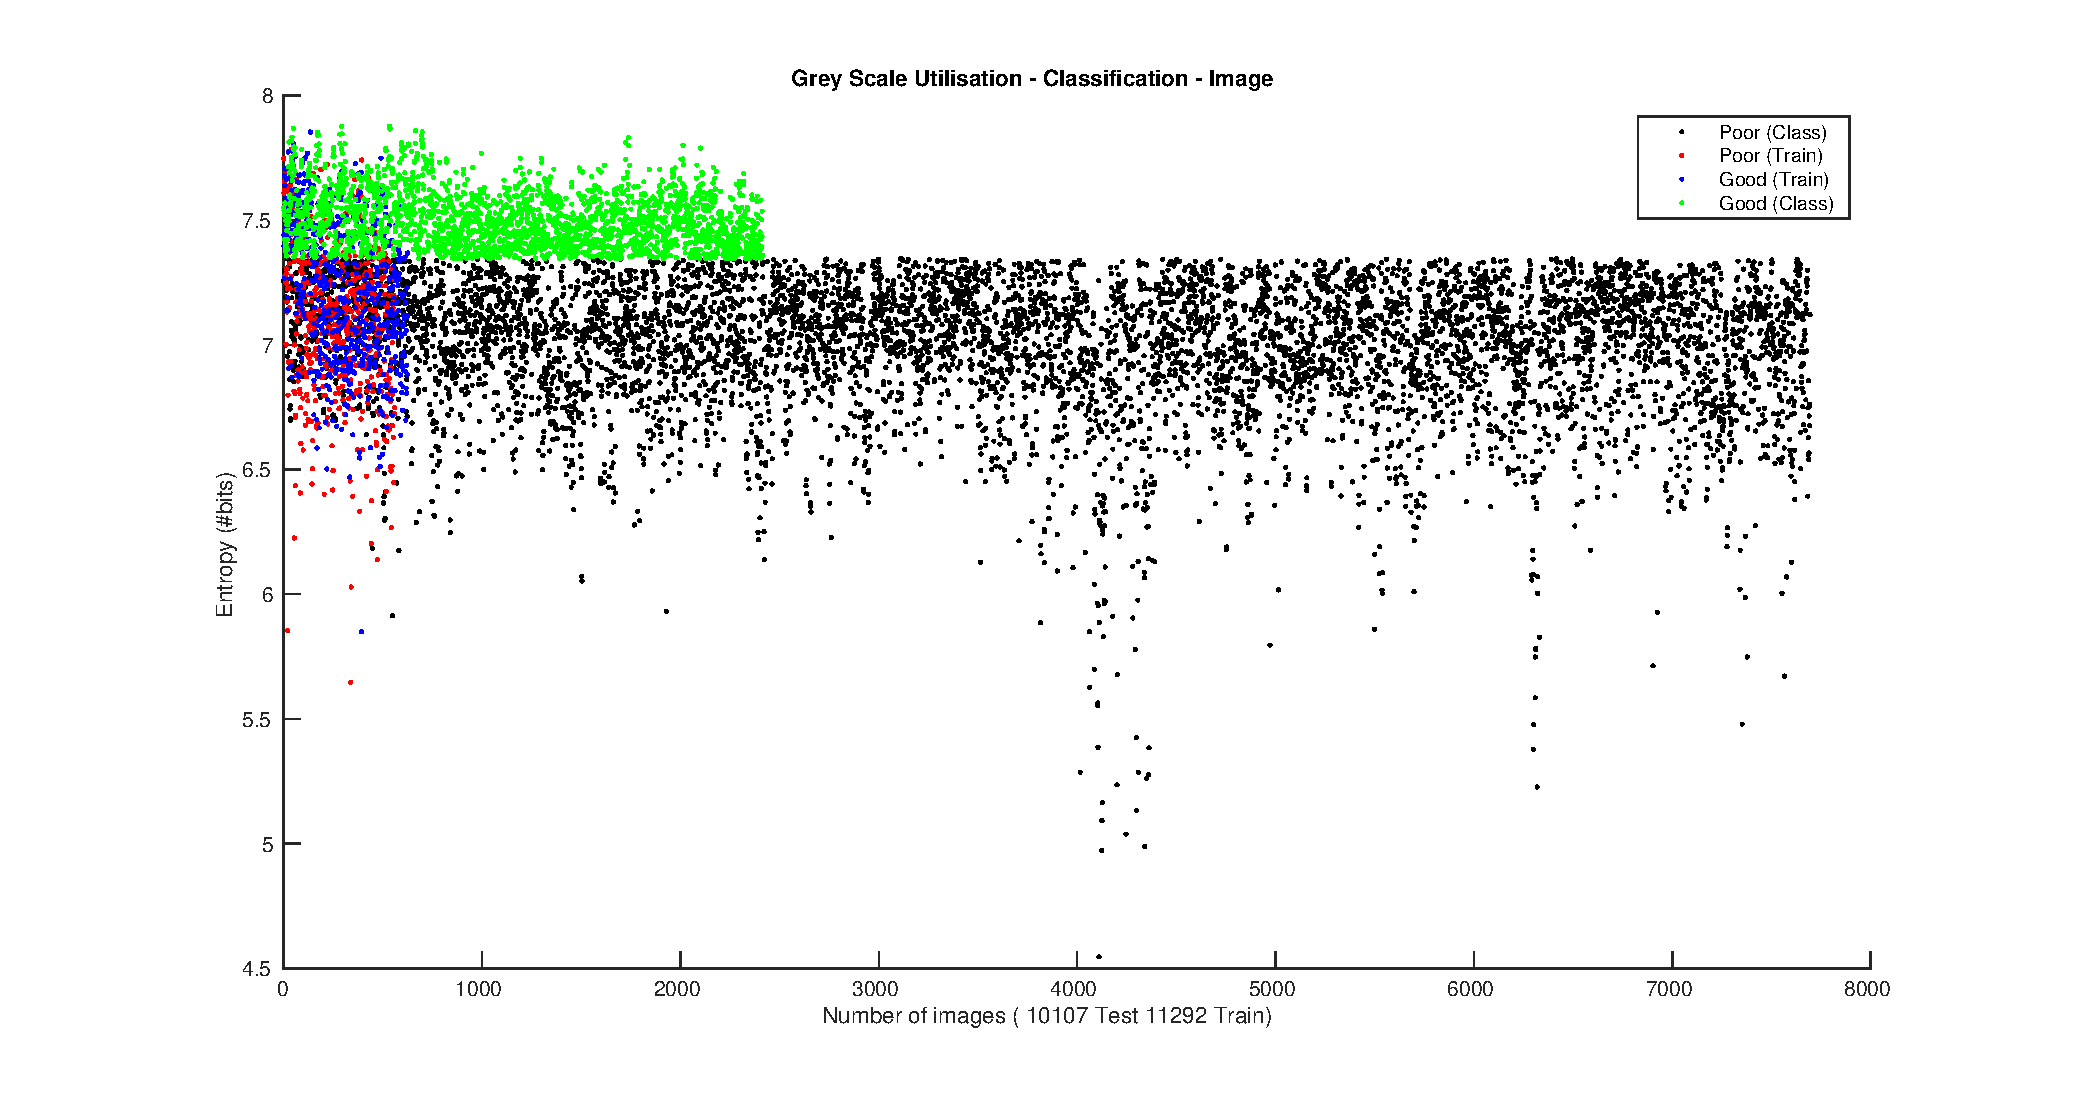
\includegraphics[width=0.9\linewidth, height=1.6cm]{pics/biqa_clas_gsu}
		\caption{Res. of class. using BIQA GSU}
		\label{fig:clas_gsu}
	\end{minipage}
\end{figure}
\begin{figure}
	\begin{minipage}{0.48\linewidth}
		\centering
		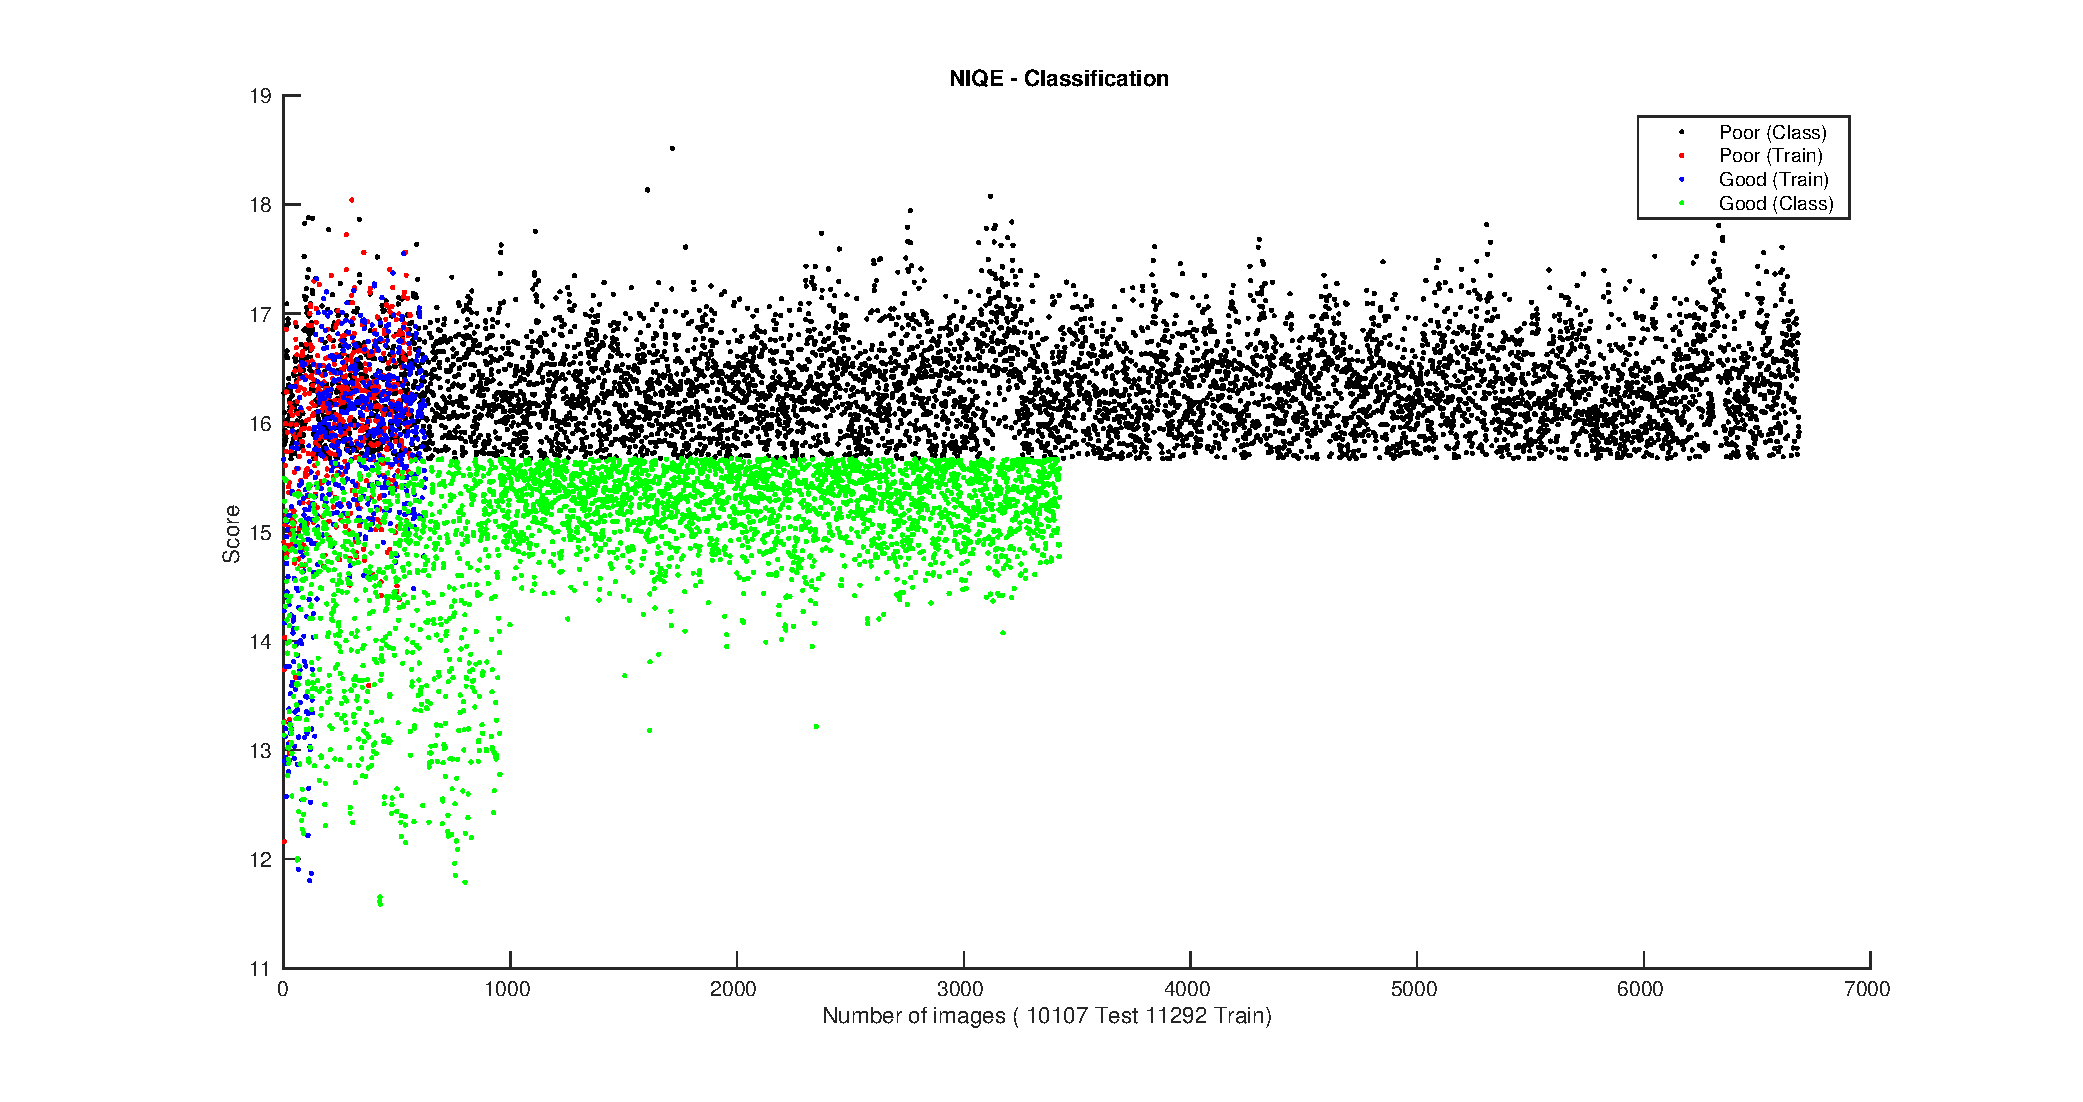
\includegraphics[width=0.9\linewidth, height=1.6cm]{pics/biqa_clas_niqe}
		\caption{Res. of class. using BIQA NIQE}
		\label{fig:clas_niqe}
	\end{minipage}
	\hfill
	\begin{minipage}{0.48\linewidth}
		\centering
		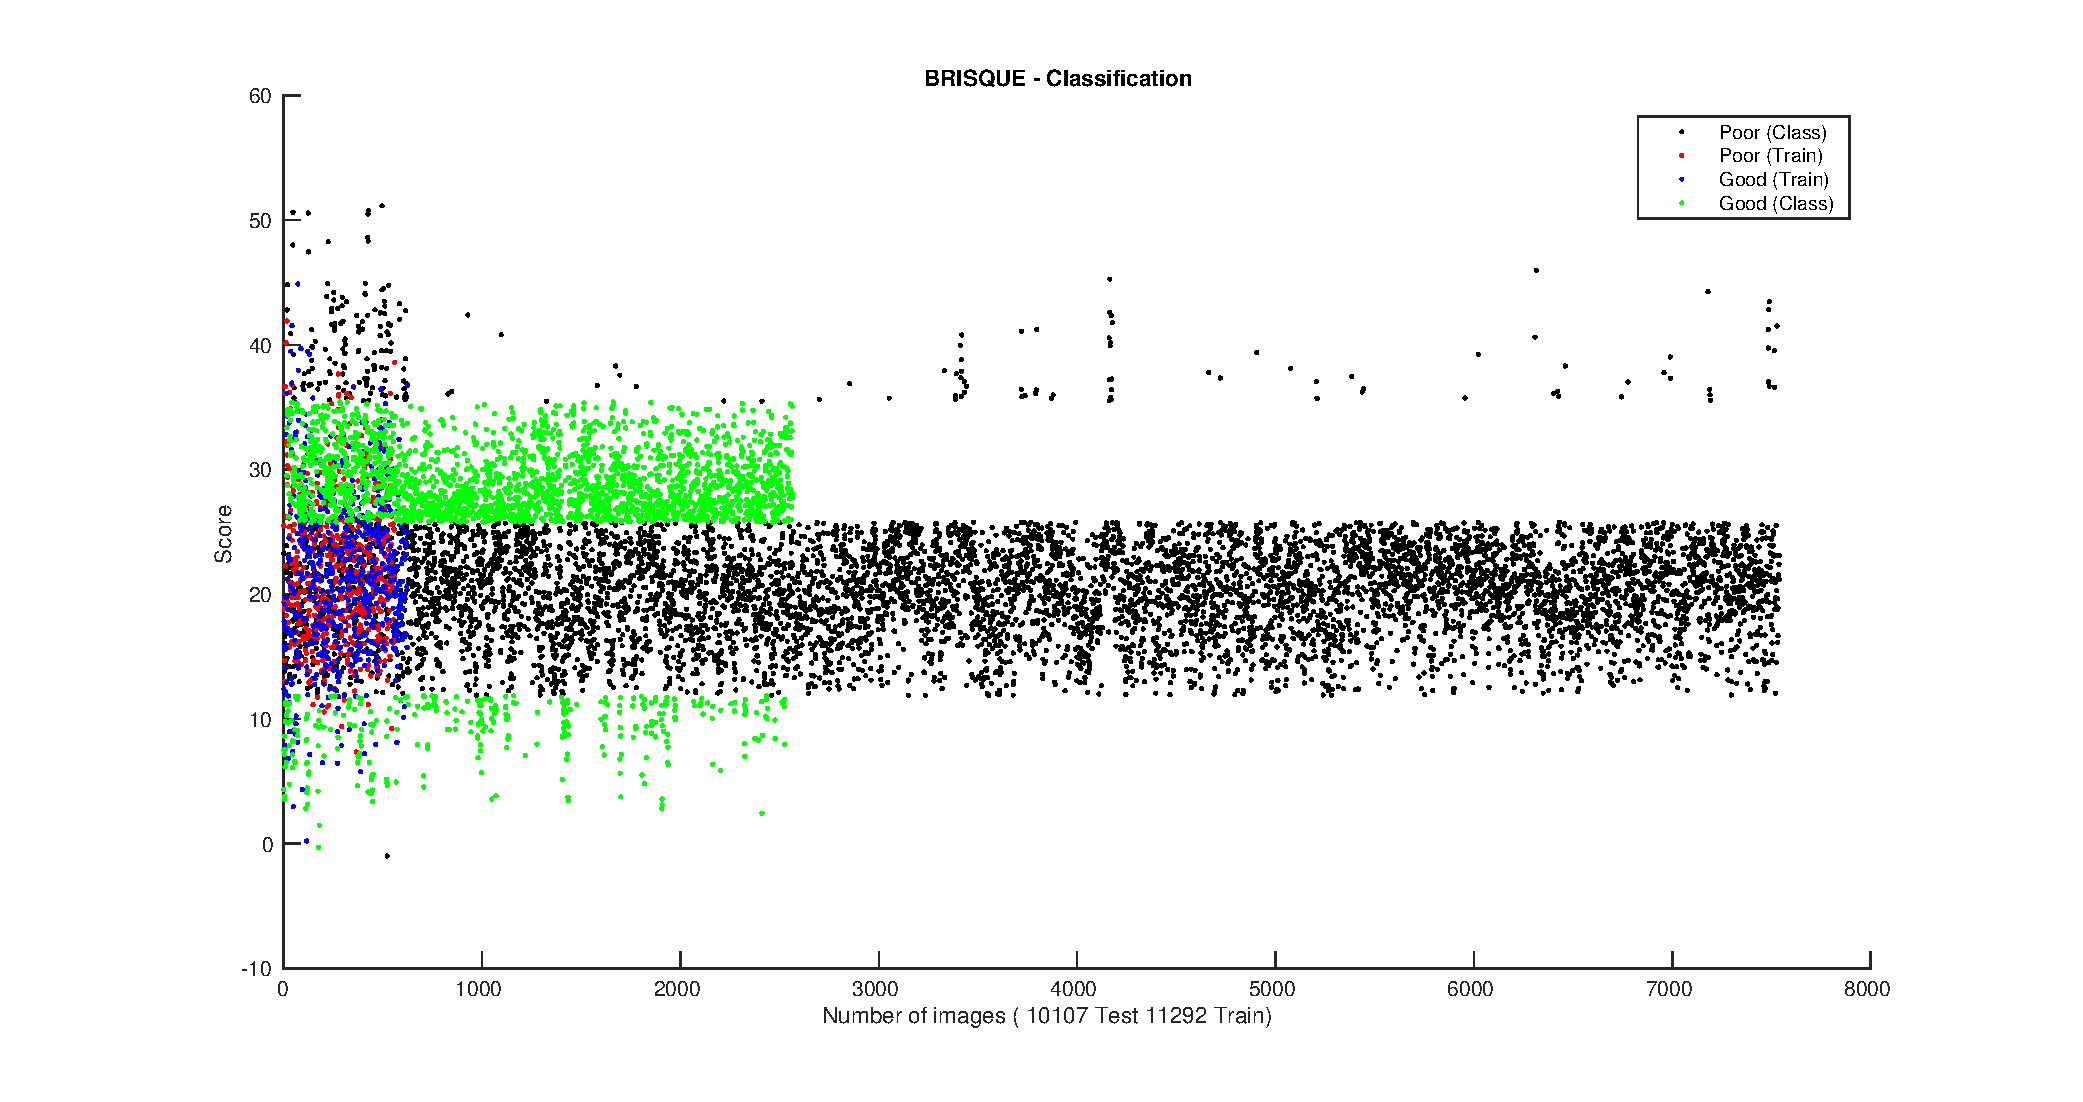
\includegraphics[width=0.9\linewidth, height=1.6cm]{pics/biqa_clas_brisque}
		\caption{Res. of class. using BIQA BRISQUE}
		\label{fig:clas_brisque}
	\end{minipage}
\end{figure}
\begin{figure}
	\begin{minipage}{0.48\linewidth}
		\centering
		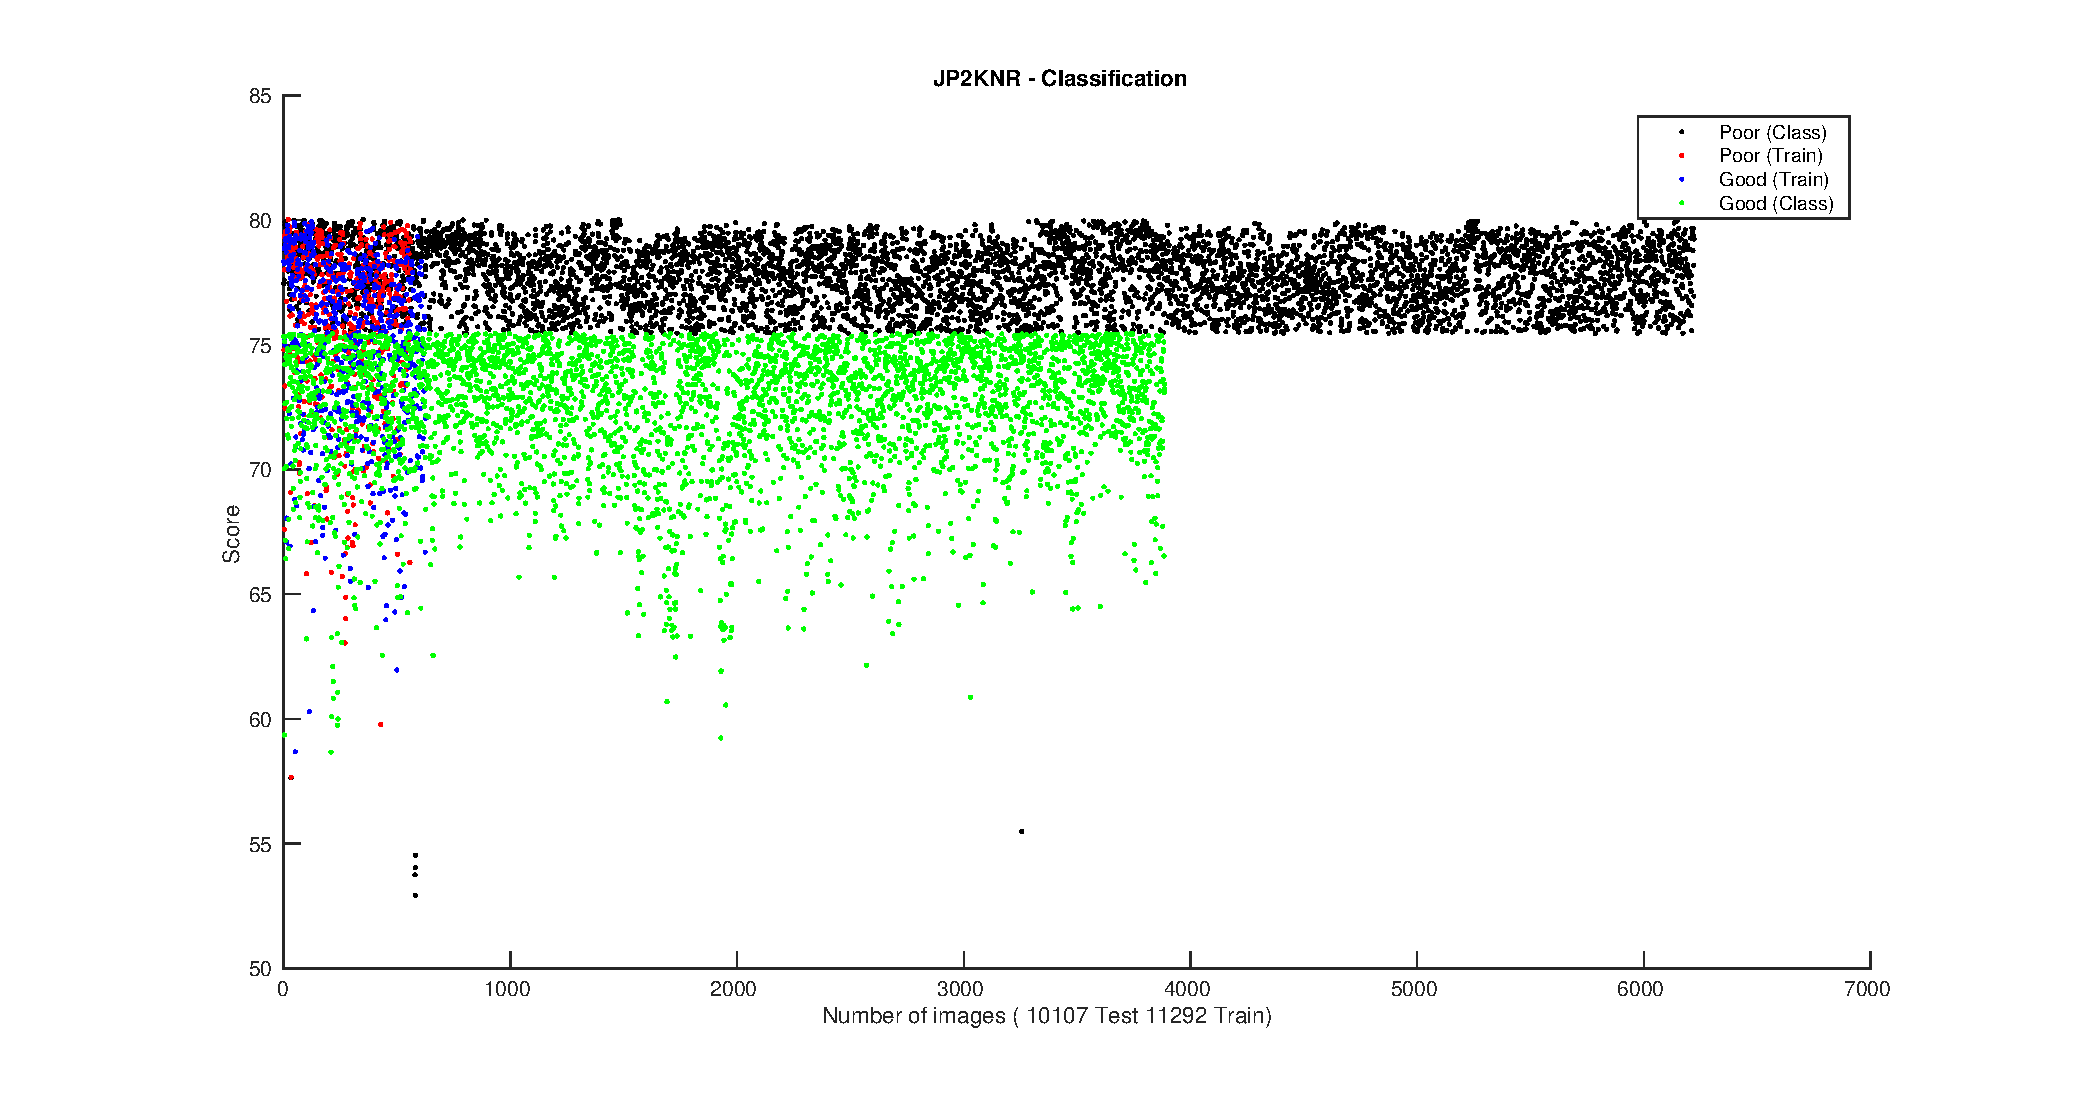
\includegraphics[width=0.9\linewidth, height=1.6cm]{pics/biqa_clas_jp2knr}
		\caption{Res. of class. using BIQA JP2KNR}
		\label{fig:clas_jp2knr}
	\end{minipage}
	\hfill
	\begin{minipage}{0.48\linewidth}
		\centering
		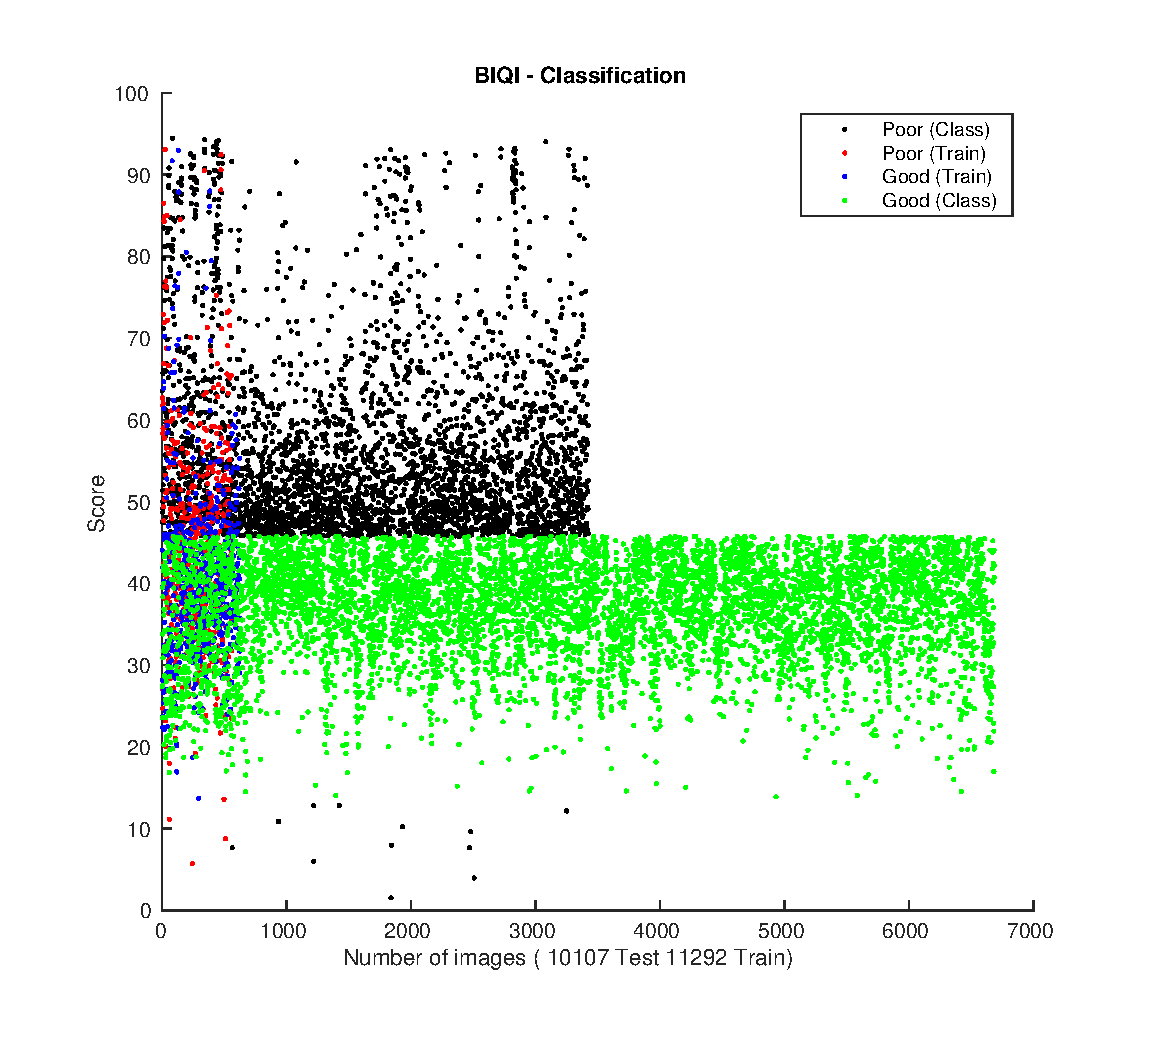
\includegraphics[width=0.9\linewidth, height=1.6cm]{pics/biqa_clas_biqi}
		\caption{Res. of class. using BIQA BIQI}
		\label{fig:clas_biqi}
	\end{minipage}
\end{figure}
\pagebreak



\subsection{Result}
\label{sec:res}
After inspecting the individual metrics ability to perform classification based
on the 625/560 images used for training is quite well.  During my initial
analysis of the metric distributions before classification, I believed several
of the would do well.  The resulting scatter plots from the classifications
shows that the 3rd party tools work very well on classifying the images as good
or bad with minimal training.

The 1185 images used for training represent a portion of ~10.5\%\ of all images
used. This 5.5\%\ "good" images was used to train against "good" image metrics,
while 4.9\%\ "bad" images was used to train against "bad" image metrics.

This is quite small number and should be increased in future tests to verify the
results.

The metrics which performed good on classification was, BIQA Iris-Pupil contrast
metric (fig. \ref{fig:clas_ipc}), BIQA Iris-Sclera contrast metric (fig.
\ref{fig:clas_isc}) BIQA Pupil-iris ratio metric(fig. \ref{fig:clas_pir}), BIQA
GSU metric(fig. \ref{fig:clas_gsu}), NIQE\cite{niqe} (fig. \ref{fig:clas_niqe}),
BRISQUE\cite{brisque} (fig. \ref{fig:clas_brisque}), JP2KNR\cite{jp2knr}(fig.
\ref{fig:clas_jp2knr}), and BIQI\cite{biqi} (fig. \ref{fig:clas_biqi}).

The result is that this subset of metrics of "good" metrics are very likely to
be applicable for images captured in the visible wavelength spectrum.  The
remaining metrics are due to poor implementation, or that the data not usable
for classifying images of irises in the visible wavelength spectrum.

There was many hinders in order to perform this project,
OSIRISv4.1\cite{osiris}, which seems to have some bugs.  Segmentation
fault, unable to discovering pupil and iris boundaries on high resolution and
high quality images.  This begs the question whether OSIRISv4.1 in itself is
applicable for performing pupil and iris discovery as well as segmentation on
images in visible wavelength spectrum.  The last was the state of the data sets,
many images don't have irises visible in the image, way to occluded or otherwise
degraded.





\begin{table}[h]
\begin{minipage}{0.48\linewidth}
	\centering
	\begin{tabular}{l  r r r}
		\bf{Metric} 								& \bf{Good} & \bf{Bad} \\\hline
		 IQA  Iris Area							& 34   & 	 10073\\
		 IQA  Iris angle offset			& 9056 & 		1051\\
		 IQA  Focus									& 216  &  	9891\\
		 IQA  Motion Magnitude 			& 138  & 		9969\\
		 IQA  Pupil dilation				& 0    & 	 10107\\
		 BIQA  Usable iris area			& 4267 & 		5840\\
		 BIQA Iris-Pupil Contrast		& 6465 & 		3642\\
		 BIQA Iris-Sclera contrast	& 7535 & 		2572\\
		 BIQA Pupil-Iris Ratio			& 6266 & 		3841\\
		 BIQA GSU										& 2413 & 		7694\\
		 BIQA NIQE									& 3423 & 		6684\\
		 BIQA BRISQUE								& 2567 & 		7540\\
		 BIQA JP2KNR								& 3886 & 		6221\\
		 BIQA BIQI									& 6684 & 		3423\\\hline
	\end{tabular}
	\caption{Individual classification summary}
	\label{tab:indclas}
\end{minipage}
\hfill
\begin{minipage}{0.48\linewidth}
	\centering
	\begin{tabular}{l  r r r}
		\bf{Metric} 								& \bf{Good} 	& \bf{Poor} 			\\\hline
		 IQA  Iris Area							&  						&	\checkmark   	\\
		 IQA  Iris angle offset			&  						& \checkmark 		\\
		 IQA  Focus									&   					& \checkmark   	\\
		 IQA  Motion Magnitude 			&   					& \checkmark  	\\
		 IQA  Pupil dilation				&    					& \checkmark  	\\
		 BIQA  Usable iris area			&  						& \checkmark 		\\
		 BIQA Iris-Pupil Contrast		& \checkmark  & 		\\
		 BIQA Iris-Sclera contrast	& \checkmark  & 		\\
		 BIQA Pupil-Iris Ratio			& \checkmark  & 		\\
		 BIQA GSU										& \checkmark  & 		\\
		 BIQA NIQE									& \checkmark  & 		\\
		 BIQA BRISQUE								& \checkmark  & 		\\
		 BIQA JP2KNR								&	\checkmark  & 		\\
		 BIQA BIQI									& \checkmark  & 		\\\hline
	\end{tabular}
	\caption{Conclusion to metric applicability}
	\label{tab:appl}
\end{minipage}
\end{table}


\section{Conclusion}
\label{sec:conc}
In this paper I have explored and developed tools for extracting and evaluating
the applicability of using certain metrics to ascertain the quality and ability
to classify images of the periocular region, captured in the visible wavelength
spectrum.

I concentrated on three 3rd party tools, the metrics proposed by Hugo
Proenca\cite{hugo} and metrics dictated by the ISO standard 29794-6\cite{iso}.

From the metrics proposed by these I selected the following subset of metrics,
see table \ref{tab:appl}, which should explored and further tested.  The table
summarises my conclusion of which metrics can be proposed as "good" for images
captured in the visible wavelength spectrum.

However, this conclusion still needs to be further investigated because of the
way the tools has been developed and any errors which may have been made,
especially by the OSIRISv4.1\cite{osiris}.  However, in consideration to this,
my conclusion is still, with the results shown, that table \ref{tab:appl} 
summarises which metrics are most applicable.



\section{Future work}

\paragraph{OSIRISv4.1}
Trying to process large data sets, long list of images, OSIRISv4.1 has a severe 
memory leak on large data sets. Which currently must be mitigated by splitting 
the list or run a program on the side which initialises OSIRIS for every image.

While automating the OSIRISv4.1 I encountered errors where the current image
failed, but no errors was issued and errors was given for the next images, which
processed correctly.  This caused some issues during my automation process.
This was mitigated by avoiding error handling all together and creating a second
script which is run after all OSIRISv4.1 processes has ended.


\paragraph{Further development of BIQA and IQA}
Current development of this project and its tools is serialised tasks in Matlab
which takes a long time to run.  Processing 12.000 images on a Debian 7 Wheezy,
using 6GB RAM and four 2.3GHz Cores takes approximately 24 hours with IQA and 18
hours with BIQA.  Pre-processing the images using the automated python script
which tries up to three configurations per image takes also approximately 3-4
hours using OSIRISv4.1.

All of this has to be streamlined into a multihreaded application in order to
reduce the time spent idling. With a tailored application for this, the time
spent processing the entire data set should be shortened to maximum a couple of
hours.




%\section*{Acknowledgements}
I would like to thank Kiran Bylappa Raja from the Norwegian Biometric Laboratory
at NISlab for his supervision and guidance during this project.


\bibliographystyle{lnig}
\bibliography{main}



% that's all folks
\end{document}


